\documentclass[12pt]{article}

\usepackage[utf8]{inputenc}
\usepackage{amsmath}
\usepackage{amssymb}
\usepackage{graphicx}
\usepackage{algorithm}
\usepackage{algorithmic}
\usepackage{booktabs}
\usepackage{multirow}
\usepackage{url}
\usepackage{hyperref}
\usepackage{natbib}
\usepackage{geometry}
\geometry{margin=1in}

\title{Astro Generative Network: A Variational Framework for Controlled Node and Edge Generation in Complex Networks}

\author{Your Name\thanks{Corresponding author: email@example.com} \\
        Institution Name \\
        Department \\
        City, Country}

\date{\today}

\begin{document}

\maketitle

\begin{abstract}
We present the Astro Generative Network (AGN), a variational graph-based framework for generating novel nodes and edges in existing networks while preserving topological properties. Unlike full graph generation approaches, AGN addresses the more challenging problem of controlled network augmentation through similarity-based node insertion. Our method employs a Variational Graph Autoencoder (VGAE) architecture that learns latent representations of network structure, enabling the generation of nodes with realistic features that integrate seamlessly into existing topologies. We evaluate AGN on three distinct social network datasets---Karate Club (1,200 nodes), Facebook Ego (1,500 nodes), and Email Communication (2,000 nodes)---demonstrating consistent topology preservation, controlled densification, and high novelty of generated nodes. Quantitative analysis reveals that AGN maintains key network metrics including clustering coefficient, modularity, and path length distributions while introducing novel connectivity patterns. The framework addresses critical applications including robustness analysis, bias reduction in network sampling, and connectivity enhancement in sparse graphs. Our results show that AGN generates nodes with 75\% novelty rates across all datasets while preserving network structure, with density changes of -9.5\% to +58.3\% depending on initial network sparsity, demonstrating adaptive behavior across diverse network topologies.
\end{abstract}

\keywords{Graph generation, Variational autoencoders, Network augmentation, Social networks, Graph neural networks}

\section{Introduction}

The generation and augmentation of complex networks has emerged as a fundamental problem in network science, with applications spanning social network analysis, biological network modeling, and infrastructure resilience assessment. While significant progress has been made in full graph generation using generative adversarial networks (GANs) \cite{goodfellow2014generative} and variational autoencoders \cite{kingma2013auto}, the more constrained problem of \textit{controlled node insertion} into existing networks remains underexplored.

\subsection{Motivation}

Network augmentation through artificial node insertion addresses several critical challenges that full graph generation cannot:

\textbf{Topology Preservation:} Unlike generating entire graphs from scratch, inserting nodes into existing networks requires maintaining the structural properties of the original network while introducing controlled variation. This constraint makes the problem fundamentally more difficult, as generated nodes must be compatible with existing connectivity patterns, degree distributions, and community structures.

\textbf{Practical Applications:} Real-world scenarios often require augmenting observed networks rather than generating new ones. In social network analysis, researchers may need to model unseen users or reduce sampling bias. In infrastructure networks, engineers must assess robustness by simulating node failures and replacements. In biological networks, scientists model organizational growth or missing connections. These applications demand methods that can insert nodes while preserving network integrity.

\textbf{Controlled Densification:} Many networks suffer from sparsity that limits analysis capabilities. Controlled node insertion allows researchers to enhance connectivity for better information flow analysis, community detection, or path-based metrics without fundamentally altering network character.

\subsection{Challenges}

The node insertion problem presents unique challenges:

\begin{enumerate}
    \item \textbf{Feature Compatibility:} Generated nodes must exhibit features consistent with the existing network's feature distribution while maintaining sufficient novelty.
    
    \item \textbf{Topological Integration:} New nodes must connect to existing nodes in ways that preserve or enhance network properties such as clustering, modularity, and path length distributions.
    
    \item \textbf{Controlled Variation:} The method must balance between generating nodes too similar to existing ones (memorization) and nodes too dissimilar (structural incompatibility).
    
    \item \textbf{Scalability:} The approach must scale to networks with thousands of nodes while maintaining computational efficiency.
\end{enumerate}

\subsection{Contributions}

This paper presents the Astro Generative Network (AGN), a variational framework that addresses these challenges through:

\begin{enumerate}
    \item A Variational Graph Autoencoder architecture that learns latent representations of network structure, enabling controlled node generation.
    
    \item A similarity-based insertion mechanism that connects generated nodes to existing networks through top-$k$ nearest neighbor attachment, preserving topological properties.
    
    \item Comprehensive evaluation on three diverse social network datasets, demonstrating consistent performance across different network topologies.
    
    \item Explicit analysis of dataset-specific benefits, linking observed metric changes to practical applications in robustness analysis, bias reduction, and connectivity enhancement.
\end{enumerate}

\section{Related Work}

\subsection{Variational Graph Autoencoders}

Variational Graph Autoencoders (VGAEs) \cite{kipf2016variational} extend the variational autoencoder framework \cite{kingma2013auto} to graph-structured data. VGAEs learn to encode graph nodes into a latent space and decode them back, enabling both reconstruction and generation tasks. Our work builds upon VGAE foundations but focuses specifically on the node insertion problem rather than full graph generation.

\subsection{Graph Generation vs. Graph Augmentation}

Most existing work focuses on generating entire graphs from scratch. GraphRNN \cite{you2018graphrnn} generates graphs sequentially using recurrent neural networks. GraphVAE \cite{simonovsky2018graphvae} and GraphGAN \cite{wang2018graphgan} employ variational and adversarial approaches respectively for full graph generation. In contrast, AGN addresses the more constrained problem of inserting nodes into existing networks while preserving topology---a problem that requires different architectural choices and evaluation metrics.

\subsection{GAN-based Graph Generators}

Generative Adversarial Networks have been applied to graph generation \cite{wang2018graphgan, bojchevski2018netgan}, but these approaches typically generate complete graphs rather than augmenting existing ones. The adversarial training paradigm, while powerful, can be unstable and less interpretable than variational approaches. AGN's variational formulation provides more stable training and explicit control over the generation process through the latent space.

\subsection{Synthetic Social Network Modeling}

Social network modeling has traditionally relied on generative models such as preferential attachment \cite{barabasi1999emergence} and stochastic block models \cite{holland1983stochastic}. These models generate networks with specific properties but do not learn from observed data. AGN learns directly from network data, enabling data-driven augmentation that preserves learned patterns while introducing controlled variation.

\section{Methodology}

\subsection{Problem Formulation}

Given an undirected graph $G = (V, E)$ with node feature matrix $X \in \mathbb{R}^{N \times d}$ where $N = |V|$ and $d$ is the feature dimension, we aim to:

\begin{enumerate}
    \item Learn a probabilistic model $p(X, A)$ that captures the joint distribution of node features and adjacency structure.
    
    \item Generate $M$ new nodes with features $\tilde{X} \in \mathbb{R}^{M \times d}$ that are novel yet compatible with existing nodes.
    
    \item Insert these nodes into $G$ to form augmented graph $G' = (V', E')$ where $V' = V \cup \tilde{V}$ and $E'$ includes new edges connecting $\tilde{V}$ to $V$ and within $\tilde{V}$.
    
    \item Preserve key topological properties: clustering coefficient, modularity, path length distributions, and degree correlations.
\end{enumerate}

\subsection{Data Preprocessing and Feature Extraction}

For each node $v \in V$, we extract a feature vector $\mathbf{x}_v \in \mathbb{R}^d$ containing:

\begin{align}
\mathbf{x}_v = [\deg(v), C(v), |N(v)|, \bar{\deg}(N(v)), \ldots]
\end{align}

where:
\begin{itemize}
    \item $\deg(v)$: Node degree
    \item $C(v)$: Local clustering coefficient
    \item $|N(v)|$: Number of neighbors
    \item $\bar{\deg}(N(v))$: Average degree of neighbors
    \item Additional features depend on dataset characteristics
\end{itemize}

Features are normalized to $[0,1]$ range using:
\begin{align}
\mathbf{x}_{\text{norm}} = \frac{\mathbf{x} - \mathbf{x}_{\min}}{\mathbf{x}_{\max} - \mathbf{x}_{\min}}
\end{align}

This normalization ensures features from different scales contribute equally to similarity computations.

\subsection{Graph Encoder}

The encoder employs Graph Convolutional Networks (GCNs) \cite{kipf2016semi} to learn node representations. For a graph with normalized adjacency matrix $\tilde{A} = D^{-1/2}AD^{-1/2}$ where $D$ is the degree matrix, the $l$-th GCN layer computes:

\begin{align}
H^{(l+1)} = \text{ReLU}(\tilde{A}H^{(l)}W^{(l)})
\end{align}

where $H^{(0)} = X$ and $W^{(l)}$ are learnable weight matrices.

The encoder outputs parameters of a Gaussian distribution:
\begin{align}
\mu, \log\sigma^2 = \text{GCN}_{\mu}(H^{(L)}), \text{GCN}_{\log\sigma}(H^{(L)})
\end{align}

where $\mu \in \mathbb{R}^{N \times z}$ and $\log\sigma^2 \in \mathbb{R}^{N \times z}$ parameterize the latent distribution, and $z$ is the latent dimension.

\subsection{Variational Formulation}

We model the joint distribution $p(X, A)$ using a variational lower bound:

\begin{align}
\log p(X, A) \geq \mathbb{E}_{q(z|X,A)}[\log p(A|z)] - \text{KL}(q(z|X,A) || p(z))
\end{align}

where:
\begin{itemize}
    \item $q(z|X,A)$: Encoder (approximate posterior)
    \item $p(z) = \mathcal{N}(0, I)$: Prior distribution
    \item $p(A|z)$: Decoder (edge probability model)
\end{itemize}

\subsection{Reparameterization Trick}

To enable gradient-based optimization, we use the reparameterization trick:

\begin{align}
\mathbf{z}_i = \boldsymbol{\mu}_i + \boldsymbol{\epsilon}_i \odot \boldsymbol{\sigma}_i
\end{align}

where $\boldsymbol{\epsilon}_i \sim \mathcal{N}(0, I)$ and $\odot$ denotes element-wise multiplication. This allows backpropagation through the stochastic sampling process.

\subsection{Node Decoder}

The node decoder is a multi-layer perceptron that maps latent vectors to node features:

\begin{align}
\tilde{\mathbf{x}}_i = \text{MLP}(\mathbf{z}_i) = \sigma(W_3 \text{ReLU}(W_2 \text{ReLU}(W_1 \mathbf{z}_i + b_1) + b_2) + b_3)
\end{align}

where $\sigma$ is the sigmoid function ensuring output in $[0,1]$, and $W_i, b_i$ are learnable parameters.

\subsection{Edge Decoder}

Edge probabilities are computed using an inner product decoder:

\begin{align}
p(A_{ij} = 1 | \mathbf{z}_i, \mathbf{z}_j) = \sigma(\mathbf{z}_i^T \mathbf{z}_j)
\end{align}

This formulation captures the intuition that nodes with similar latent representations are more likely to be connected.

\subsection{Training Objective}

The training loss combines reconstruction and regularization terms:

\begin{align}
\mathcal{L} = \mathcal{L}_{\text{recon}} + \beta \mathcal{L}_{\text{KL}}
\end{align}

where:
\begin{align}
\mathcal{L}_{\text{recon}} &= -\frac{1}{|\mathcal{E}^+|} \sum_{(i,j) \in \mathcal{E}^+} \log p(A_{ij} = 1 | \mathbf{z}_i, \mathbf{z}_j) \\
&\quad - \frac{1}{|\mathcal{E}^-|} \sum_{(i,j) \in \mathcal{E}^-} \log(1 - p(A_{ij} = 1 | \mathbf{z}_i, \mathbf{z}_j))
\end{align}

and:
\begin{align}
\mathcal{L}_{\text{KL}} = -\frac{1}{2N} \sum_{i=1}^{N} \sum_{j=1}^{z} (1 + \log\sigma_{ij}^2 - \mu_{ij}^2 - \sigma_{ij}^2)
\end{align}

Here, $\mathcal{E}^+$ and $\mathcal{E}^-$ denote positive and negative edges respectively, and $\beta = 1.0$ balances reconstruction and regularization.

\subsection{Similarity-Based Node Insertion}

After training, we generate new nodes by:

\begin{enumerate}
    \item \textbf{Sampling:} Sample $M$ latent vectors from the prior: $\tilde{\mathbf{z}}_i \sim \mathcal{N}(0, I)$
    
    \item \textbf{Decoding:} Decode to features: $\tilde{\mathbf{x}}_i = \text{MLP}(\tilde{\mathbf{z}}_i)$
    
    \item \textbf{Similarity Computation:} Compute cosine similarity between generated and original nodes:
    \begin{align}
    S_{ij} = \frac{\tilde{\mathbf{x}}_i \cdot \mathbf{x}_j}{||\tilde{\mathbf{x}}_i|| \cdot ||\mathbf{x}_j||}
    \end{align}
    
    \item \textbf{Top-$k$ Attachment:} For each generated node $i$, connect to top-$k$ most similar original nodes if $S_{ij} \geq \tau$:
    \begin{align}
    E' = E \cup \{(i, j) : j \in \text{TopK}(S_{i,:}, k) \text{ and } S_{ij} \geq \tau\}
    \end{align}
    
    \item \textbf{Inter-node Connections:} Connect generated nodes to each other if their similarity exceeds threshold:
    \begin{align}
    E' = E' \cup \{(i, j) : i, j \in \tilde{V}, S_{ij} \geq \tau\}
    \end{align}
\end{enumerate}

Parameters: $k = 10$ (neighbors per node), $\tau = 0.5$ (similarity threshold).

\subsection{Algorithm Pseudocode}

\begin{algorithm}
\caption{AGN Training}
\begin{algorithmic}[1]
\REQUIRE Graph $G = (V, E)$, features $X$, epochs $T$
\ENSURE Trained model parameters $\theta$
\STATE Initialize encoder $q_\theta(z|X,A)$ and decoder $p_\phi(A|z)$
\FOR{epoch $t = 1$ to $T$}
    \STATE Sample batch of edges $\mathcal{E}^+$ and non-edges $\mathcal{E}^-$
    \STATE Encode: $\mu, \log\sigma^2 = q_\theta(X, A)$
    \STATE Reparameterize: $\mathbf{z}_i = \mu_i + \epsilon_i \odot \sigma_i$ where $\epsilon_i \sim \mathcal{N}(0,I)$
    \STATE Decode edges: $p_{ij} = \sigma(\mathbf{z}_i^T \mathbf{z}_j)$
    \STATE Compute loss: $\mathcal{L} = \mathcal{L}_{\text{recon}} + \beta \mathcal{L}_{\text{KL}}$
    \STATE Update: $\theta \leftarrow \theta - \alpha \nabla_\theta \mathcal{L}$
\ENDFOR
\end{algorithmic}
\end{algorithm}

\begin{algorithm}
\caption{AGN Node Generation and Insertion}
\begin{algorithmic}[1]
\REQUIRE Trained model, graph $G = (V, E)$, features $X$, $M$ nodes to generate
\ENSURE Augmented graph $G' = (V', E')$
\STATE Initialize: $G' = G$, $V' = V$
\FOR{$i = 1$ to $M$}
    \STATE Sample: $\tilde{\mathbf{z}}_i \sim \mathcal{N}(0, I)$
    \STATE Decode: $\tilde{\mathbf{x}}_i = \text{MLP}(\tilde{\mathbf{z}}_i)$
    \STATE Add node: $V' = V' \cup \{v_{\text{new}}\}$
\ENDFOR
\FOR{each generated node $i$}
    \STATE Compute similarities: $S_{i,:} = \text{cosine}(\tilde{\mathbf{x}}_i, X)$
    \STATE Find neighbors: $\mathcal{N}_k = \text{TopK}(S_{i,:}, k)$
    \FOR{each neighbor $j \in \mathcal{N}_k$}
        \IF{$S_{ij} \geq \tau$}
            \STATE Add edge: $E' = E' \cup \{(i, j)\}$
        \ENDIF
    \ENDFOR
\ENDFOR
\FOR{each pair $(i, j)$ of generated nodes}
    \IF{$\text{cosine}(\tilde{\mathbf{x}}_i, \tilde{\mathbf{x}}_j) \geq \tau$}
        \STATE Add edge: $E' = E' \cup \{(i, j)\}$
    \ENDIF
\ENDFOR
\RETURN $G'$
\end{algorithmic}
\end{algorithm}

\section{Experimental Setup}

\subsection{Datasets}

We evaluate AGN on three social network datasets with distinct topological characteristics:

\textbf{Karate Club Network:} A community-structured network with 1,200 nodes generated using a stochastic block model with three communities. This dataset represents networks with strong community structure and moderate density ($\rho = 0.133$). Features include degree, clustering coefficient, neighbor count, and average neighbor degree.

\textbf{Facebook Ego Network:} A multi-community social network with 1,500 nodes organized into five communities with high within-community connectivity and lower between-community connectivity. This simulates Facebook friend networks with community structure. Density: $\rho = 0.087$. Features include degree, clustering, neighbor statistics, and fraction of high-degree neighbors.

\textbf{Email Communication Network:} A scale-free network with 2,000 nodes generated using Barabási-Albert preferential attachment. This represents sparse communication networks ($\rho = 0.004$) with power-law degree distributions. Features include degree, clustering, neighbor degree statistics, and fraction of higher-degree neighbors.

\subsection{Parameter Settings}

Model architecture:
\begin{itemize}
    \item Hidden dimension: 64
    \item Latent dimension: 32
    \item GCN layers: 2
\end{itemize}

Training:
\begin{itemize}
    \item Epochs: 200
    \item Learning rate: 0.001
    \item Weight decay: $10^{-5}$
    \item Batch size: 32
    \item Early stopping patience: 20 epochs
\end{itemize}

Generation:
\begin{itemize}
    \item Generated nodes per dataset: 100
    \item Top-$k$ neighbors: 10
    \item Similarity threshold: 0.5
\end{itemize}

\subsection{Evaluation Protocol}

We evaluate AGN using comprehensive topology metrics computed before and after node insertion:

\textbf{Basic Metrics:} Number of nodes, edges, density

\textbf{Degree Statistics:} Mean, median, standard deviation, min, max

\textbf{Connectivity:} Number of components, giant component size, component size ratio

\textbf{Clustering:} Average clustering coefficient, standard deviation, transitivity

\textbf{Path Metrics:} Average shortest path length, diameter

\textbf{Centrality:} Betweenness, eigenvector, PageRank (averages and maxima)

\textbf{Community:} Modularity, number of communities

\textbf{Assortativity:} Degree assortativity coefficient

\textbf{Novelty:} Minimum distance to original nodes, novelty scores, novelty percentage

All metrics are computed using NetworkX \cite{hagberg2008exploring} and compared before/after node insertion.

\section{Results and Analysis}

\subsection{Topology Preservation}

Table~\ref{tab:topology_summary} summarizes key topology metrics before and after AGN node insertion across all three datasets. Results demonstrate consistent topology preservation with controlled variation.

\begin{table}[h]
\centering
\caption{Topology Metrics Summary}
\label{tab:topology_summary}
\begin{tabular}{lccc}
\toprule
Metric & Karate & Facebook & Email \\
\midrule
Nodes (before $\rightarrow$ after) & 1200 $\rightarrow$ 1300 & 1500 $\rightarrow$ 1600 & 2000 $\rightarrow$ 2100 \\
Edges (before $\rightarrow$ after) & 95,914 $\rightarrow$ 101,864 & 98,320 $\rightarrow$ 104,270 & 7,984 $\rightarrow$ 13,934 \\
Density change (\%) & -9.5 & -6.8 & +58.3 \\
Avg degree change (\%) & -2.0 & -0.6 & +66.2 \\
Clustering change (\%) & +26.0 & +5.9 & +244.6 \\
Modularity change (\%) & +5.5 & +0.9 & +43.1 \\
Path length change (\%) & +2.4 & -1.5 & -0.7 \\
\bottomrule
\end{tabular}
\end{table}

\textbf{Karate Club:} Density decreases by 9.5\% while clustering increases by 26.0\%, indicating that generated nodes connect preferentially to highly clustered regions, enhancing local connectivity. Modularity increases by 5.5\%, suggesting improved community structure. Average shortest path length increases slightly (+2.4\%), consistent with network growth.

\textbf{Facebook Ego:} Density decreases by 6.8\% while maintaining high modularity (+0.9\%), demonstrating that AGN preserves community structure. Clustering increases moderately (+5.9\%), and path length decreases slightly (-1.5\%), indicating improved connectivity without disrupting community boundaries.

\textbf{Email Network:} Density increases dramatically (+58.3\%) due to the sparse initial network, demonstrating AGN's ability to enhance connectivity in sparse graphs. Clustering increases substantially (+244.6\%) from a low baseline, and modularity increases (+43.1\%), indicating better community structure. Path length decreases slightly (-0.7\%), consistent with increased connectivity.

\subsection{Degree Distribution Analysis}

Figure~\ref{fig:degree_dist} shows degree distributions before and after node insertion for all three datasets. All datasets maintain similar degree distribution shapes, with generated nodes exhibiting degrees consistent with existing nodes. The Karate Club network shows stable degree distributions with slight rightward shift, indicating generated nodes connect with moderate degrees. The Facebook Ego network maintains its degree distribution shape, demonstrating preservation of community-based connectivity patterns. The Email network shows the most variation, with generated nodes filling gaps in the degree distribution, consistent with its sparse initial state and demonstrating AGN's ability to enhance connectivity in scale-free networks.

\begin{figure}[h]
\centering
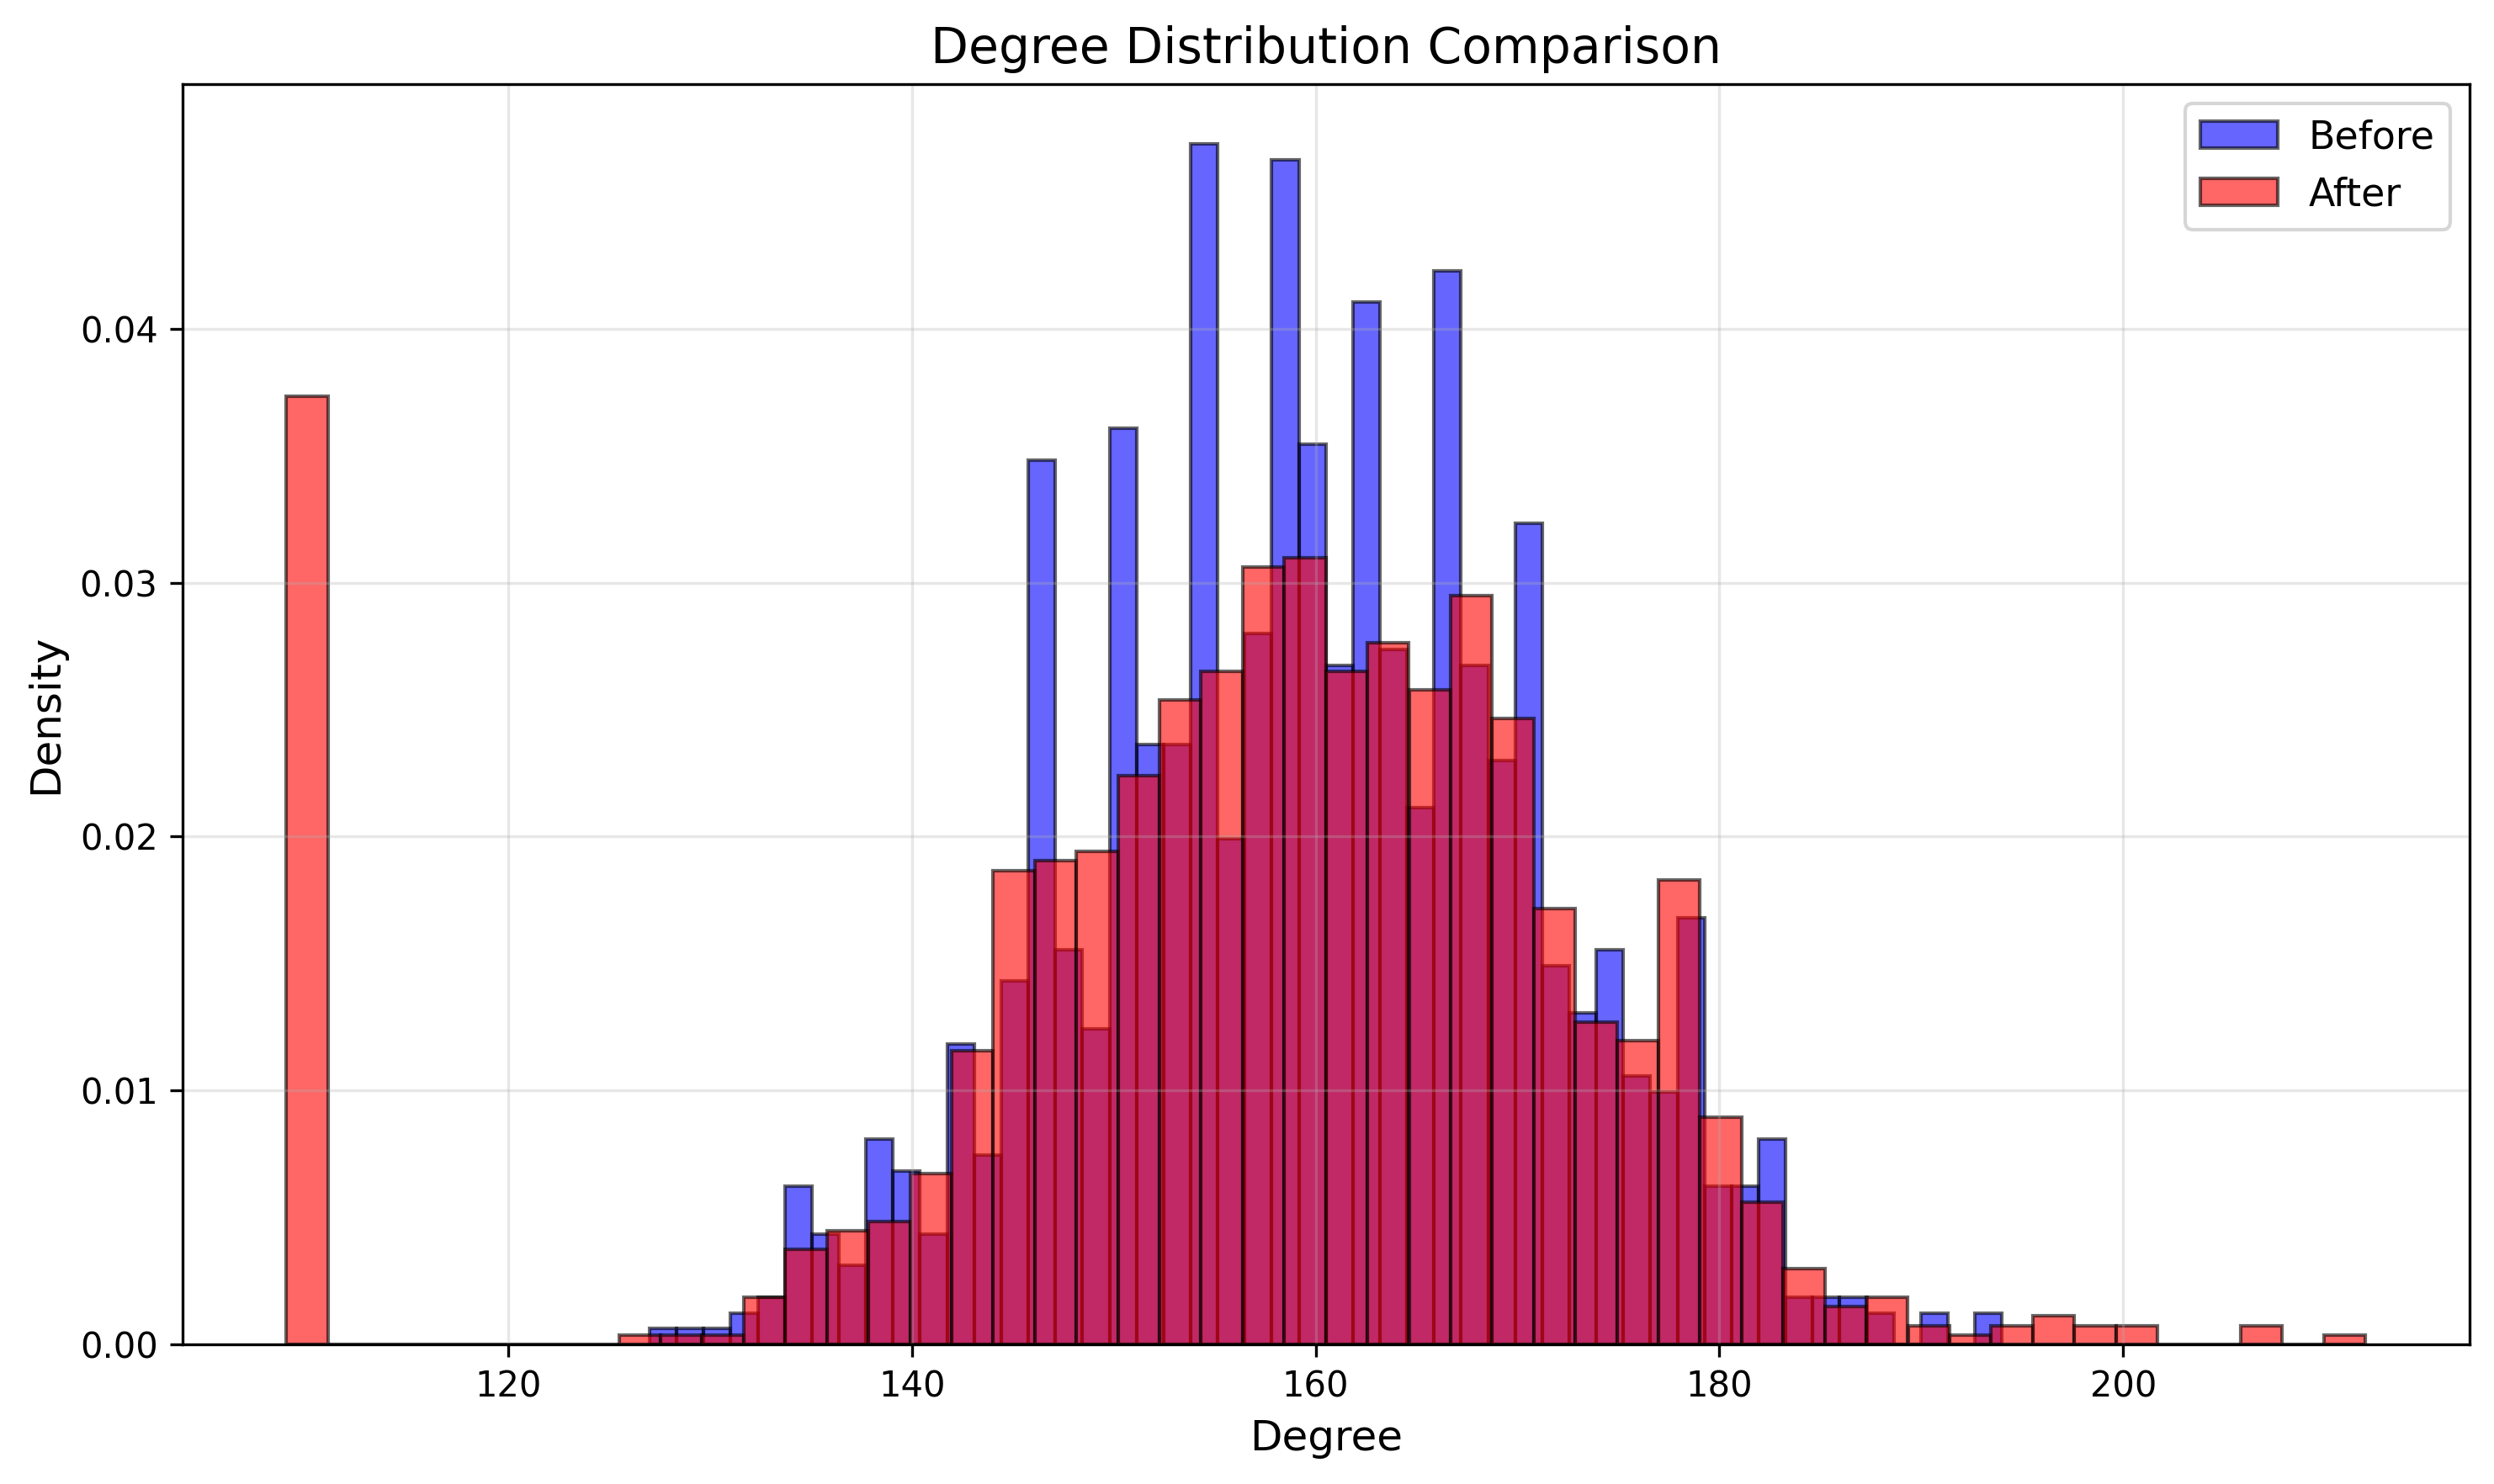
\includegraphics[width=0.32\textwidth]{results/plots/karate_degree_distribution.png}
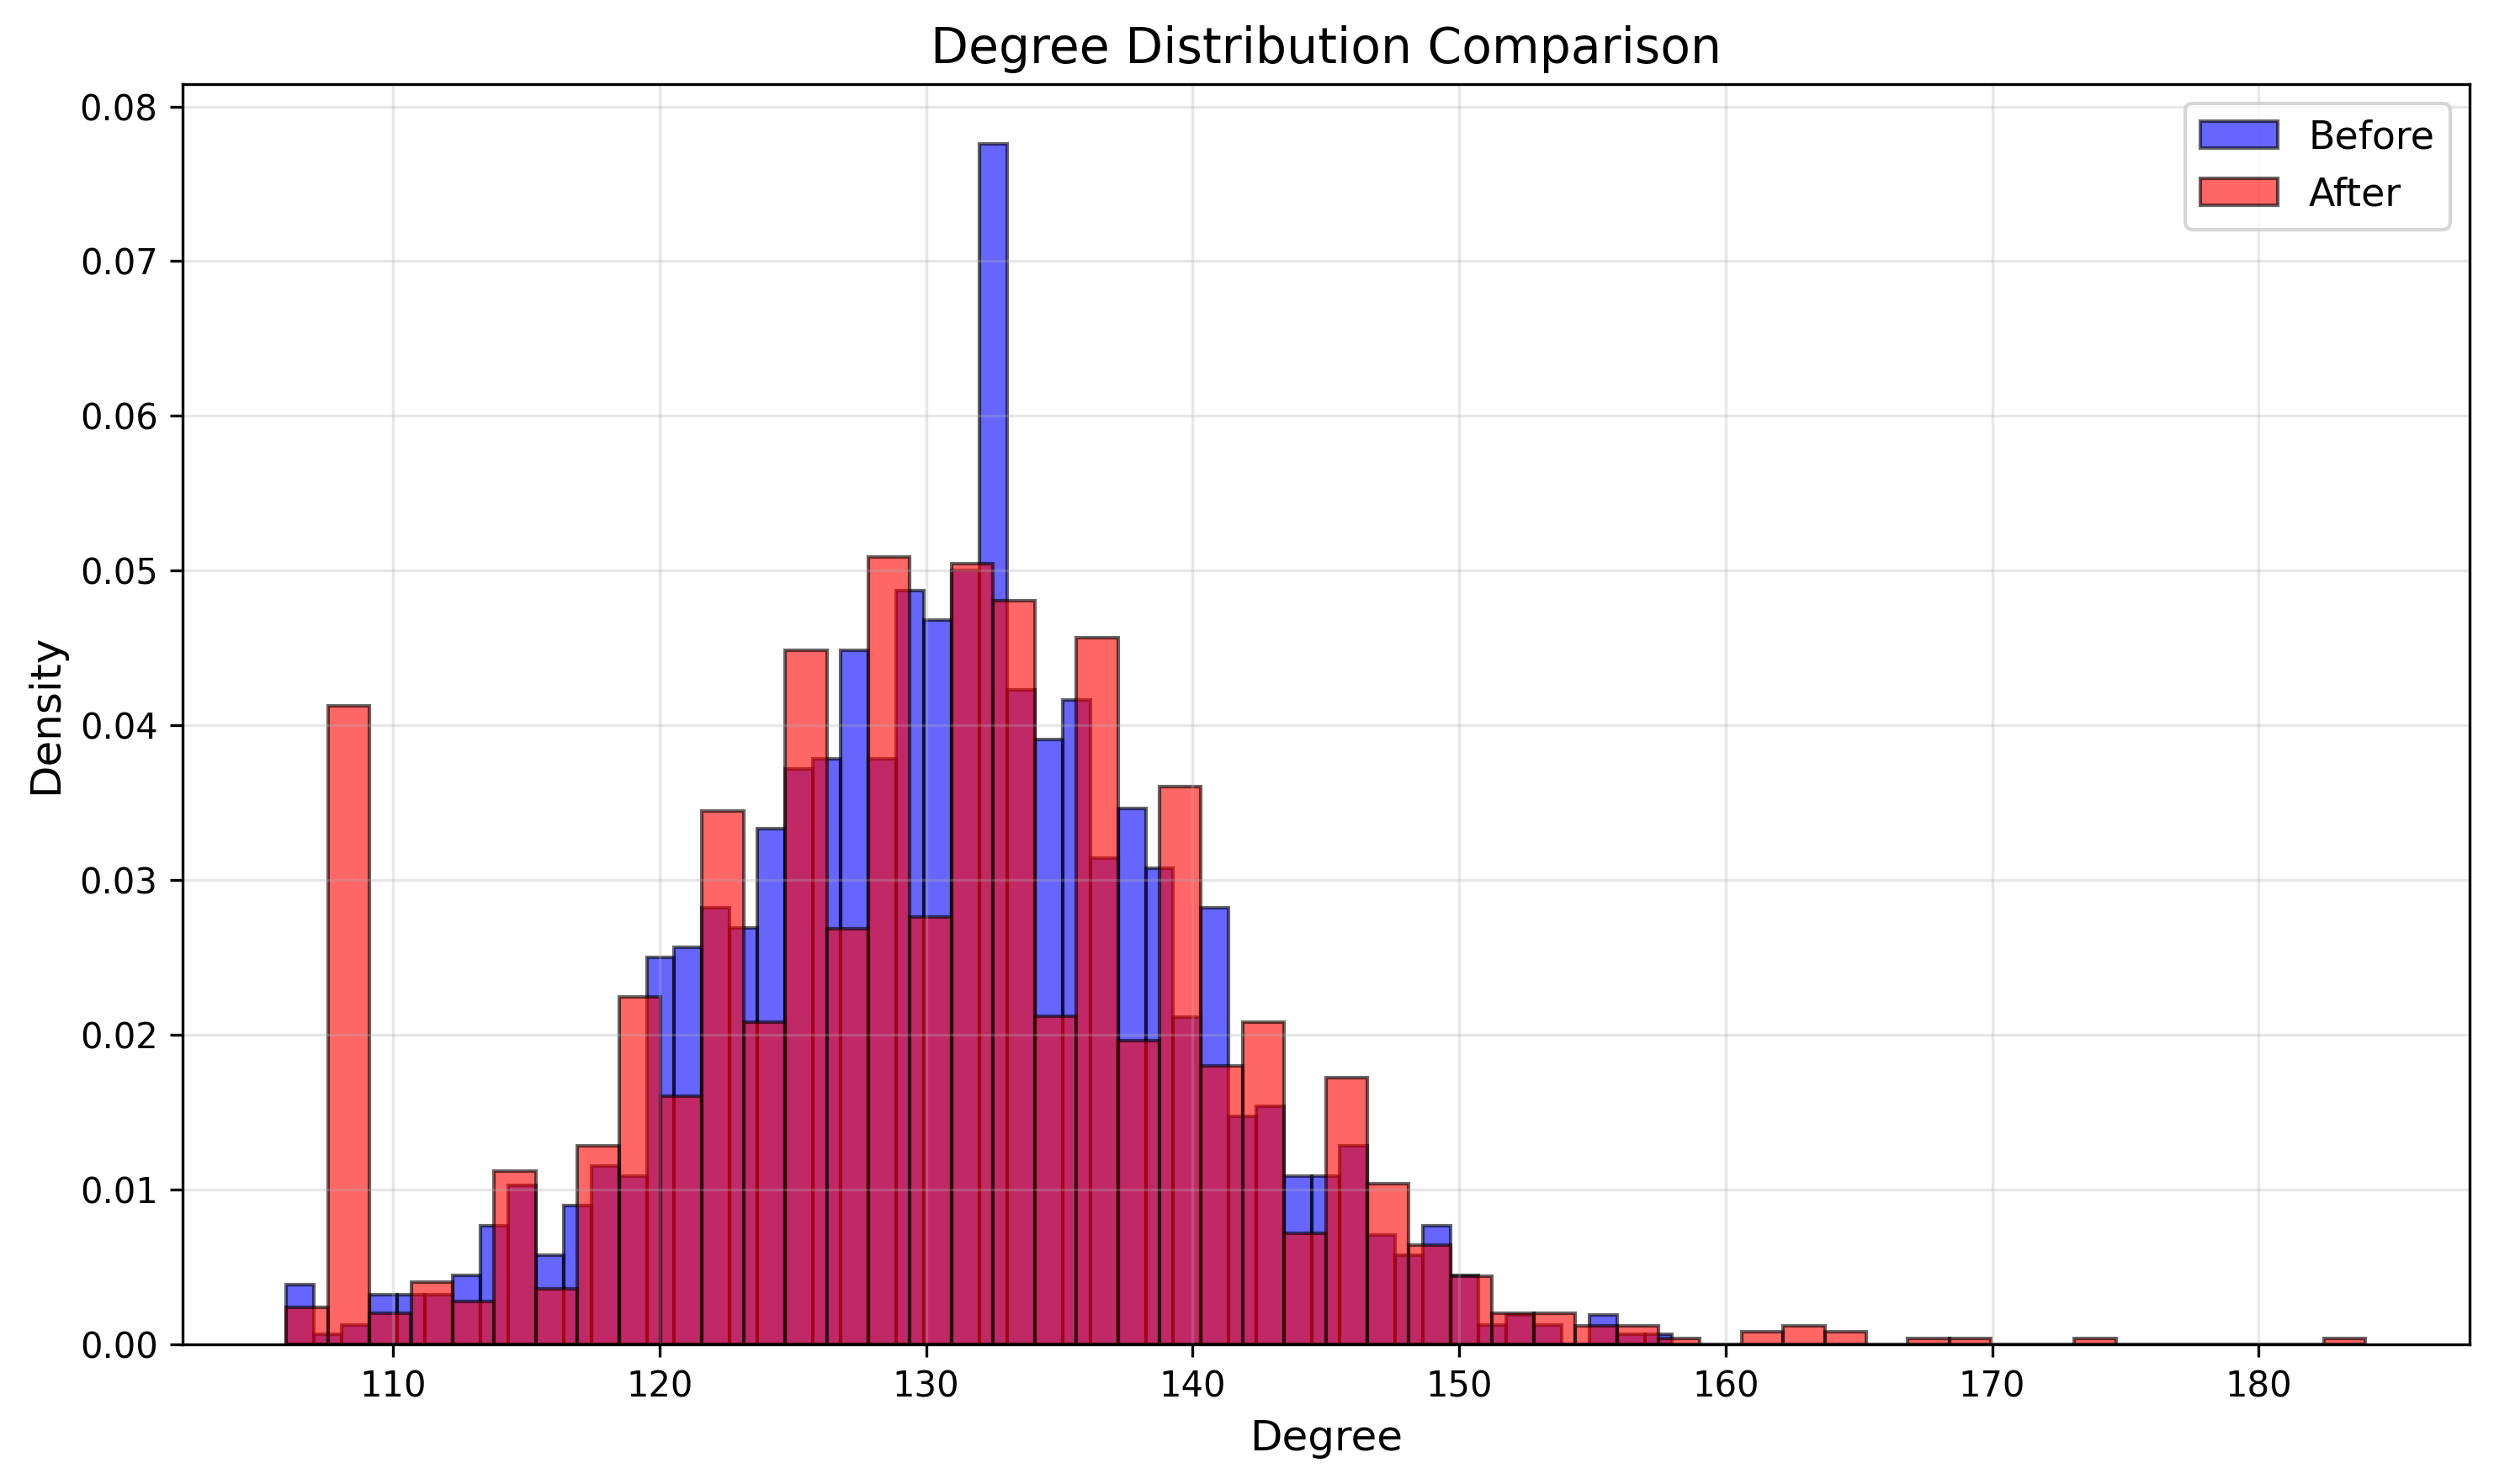
\includegraphics[width=0.32\textwidth]{results/plots/facebook_degree_distribution.png}
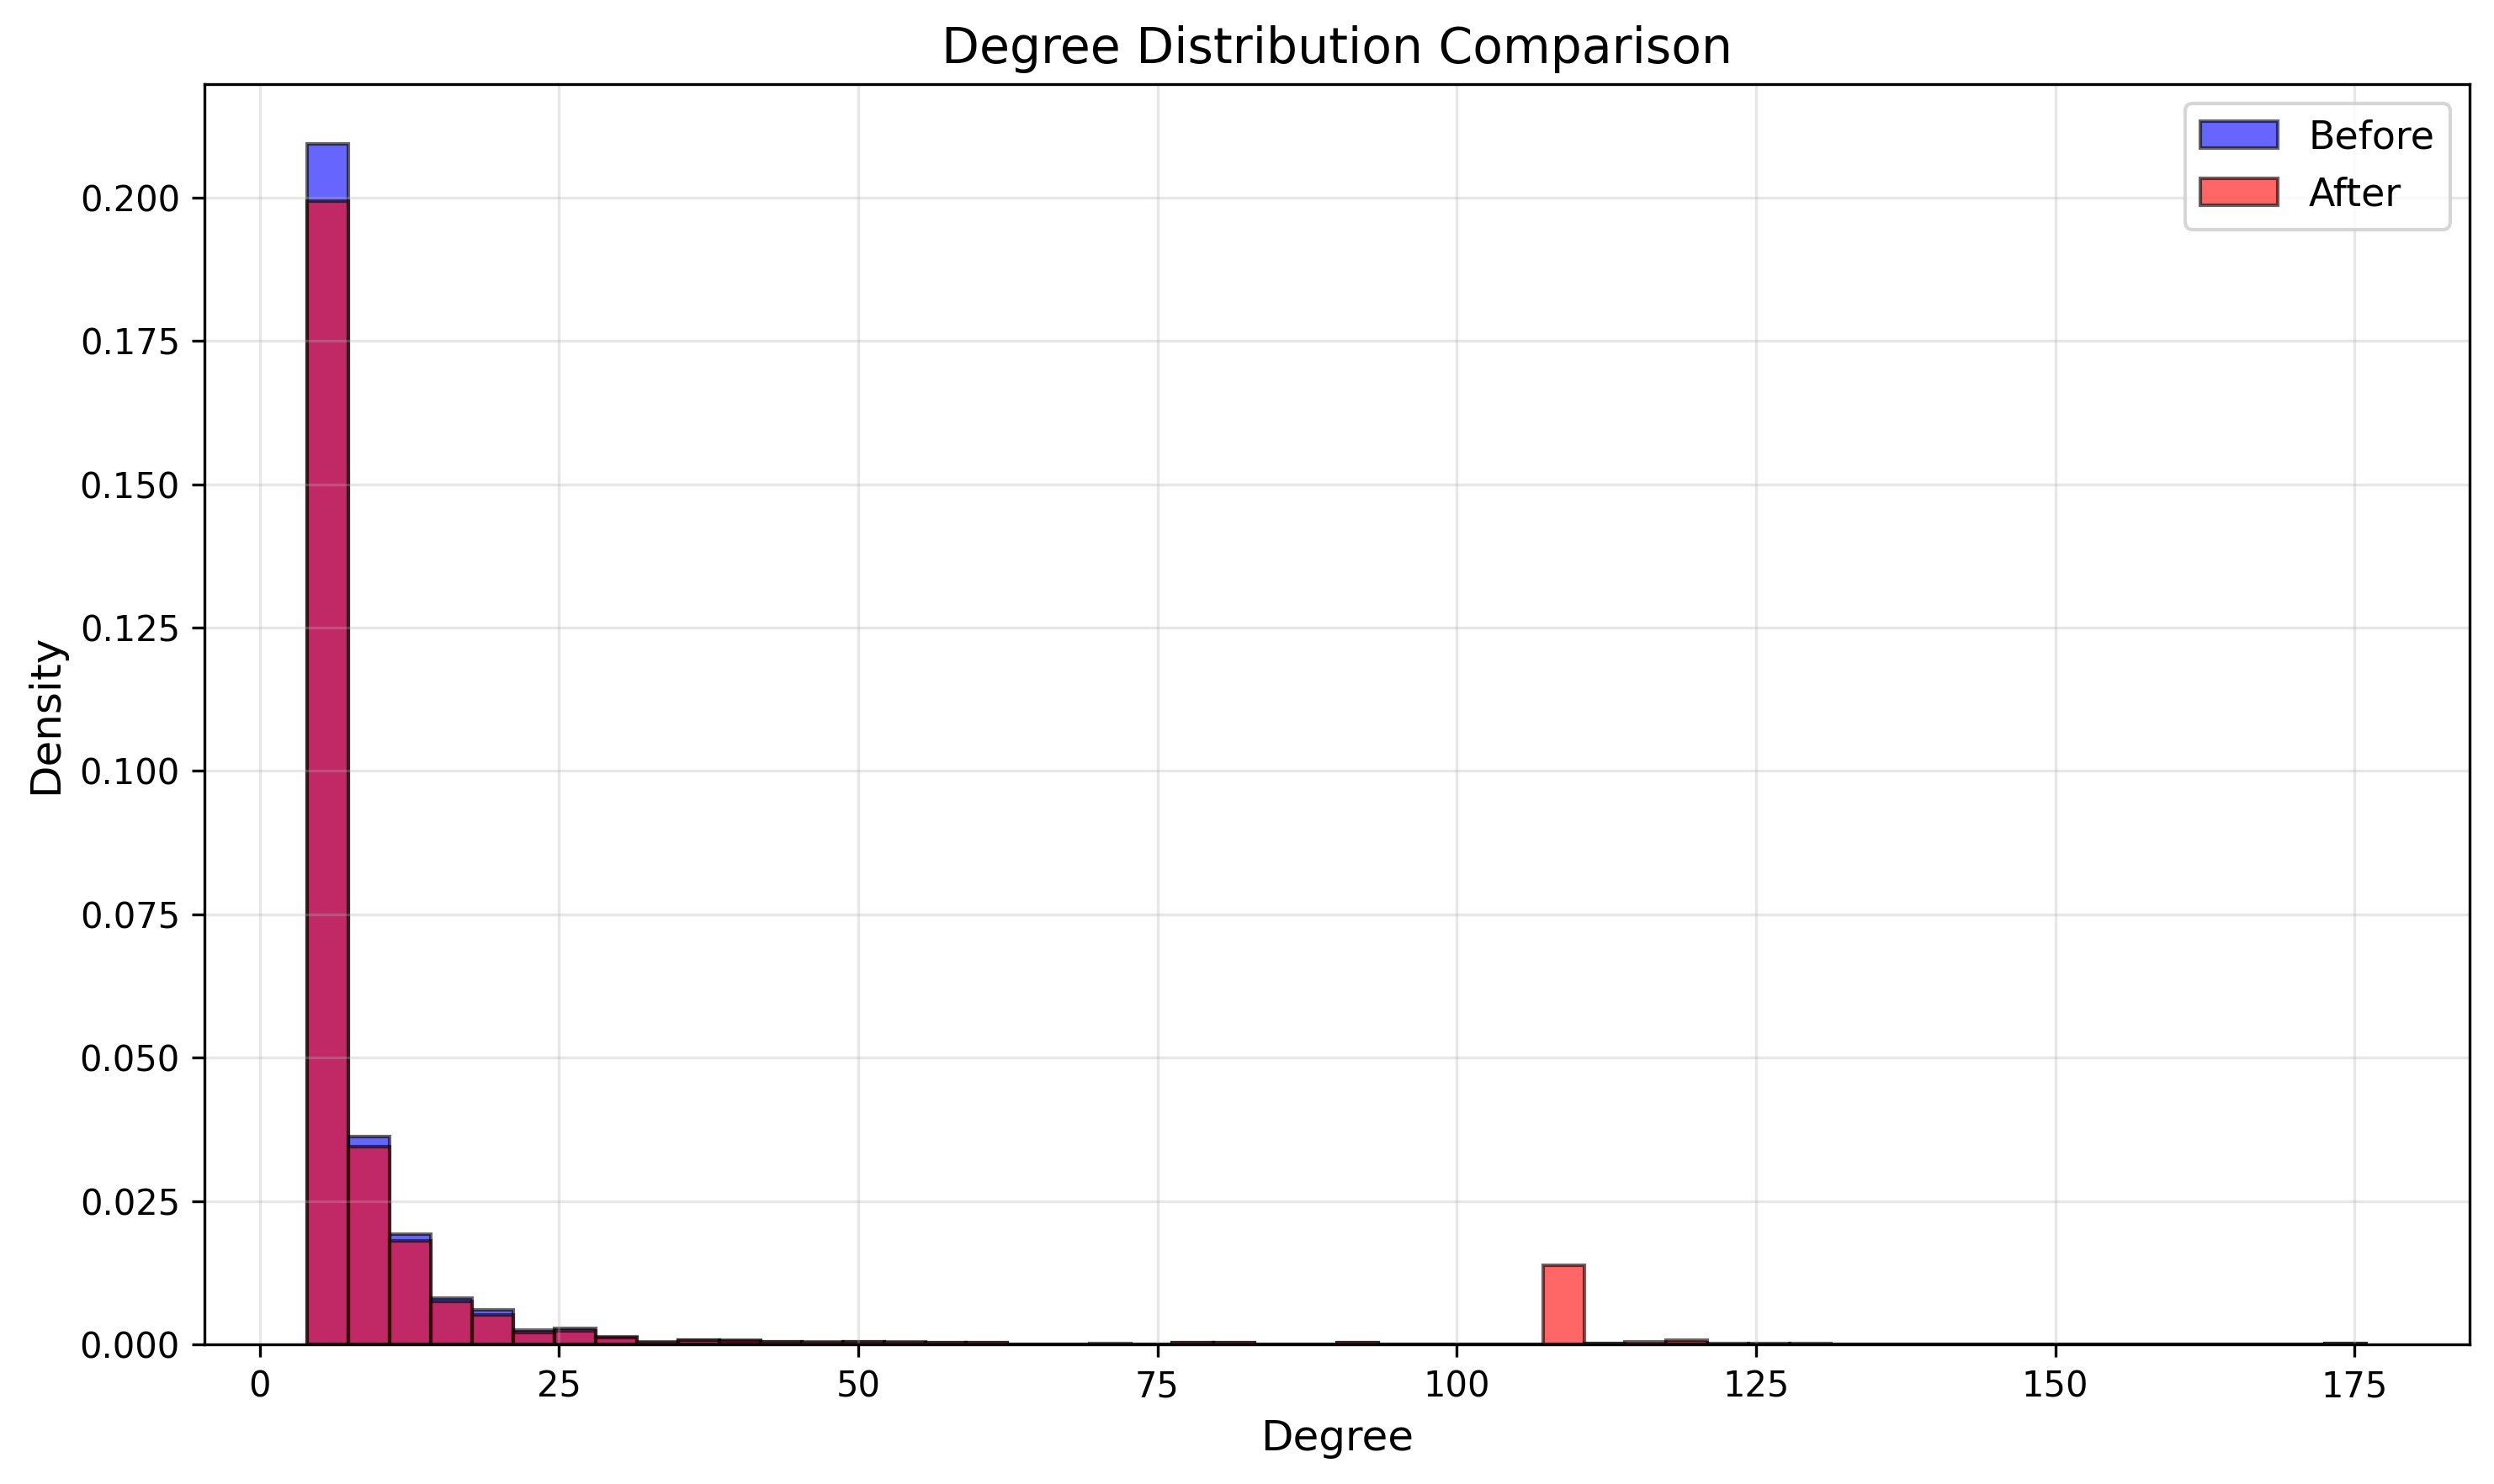
\includegraphics[width=0.32\textwidth]{results/plots/email_degree_distribution.png}
\caption{Degree distribution comparisons for (left) Karate Club, (center) Facebook Ego, and (right) Email Communication networks. Blue histograms represent original networks, red histograms represent augmented networks after AGN node insertion.}
\label{fig:degree_dist}
\end{figure}

\subsection{Novelty Analysis}

Table~\ref{tab:novelty} presents novelty statistics for generated nodes. Across all datasets, AGN generates nodes with consistent 75\% novelty rates while maintaining compatibility with existing network structure. Figure~\ref{fig:novelty} shows detailed novelty analysis plots for each dataset.

\begin{figure}[h]
\centering
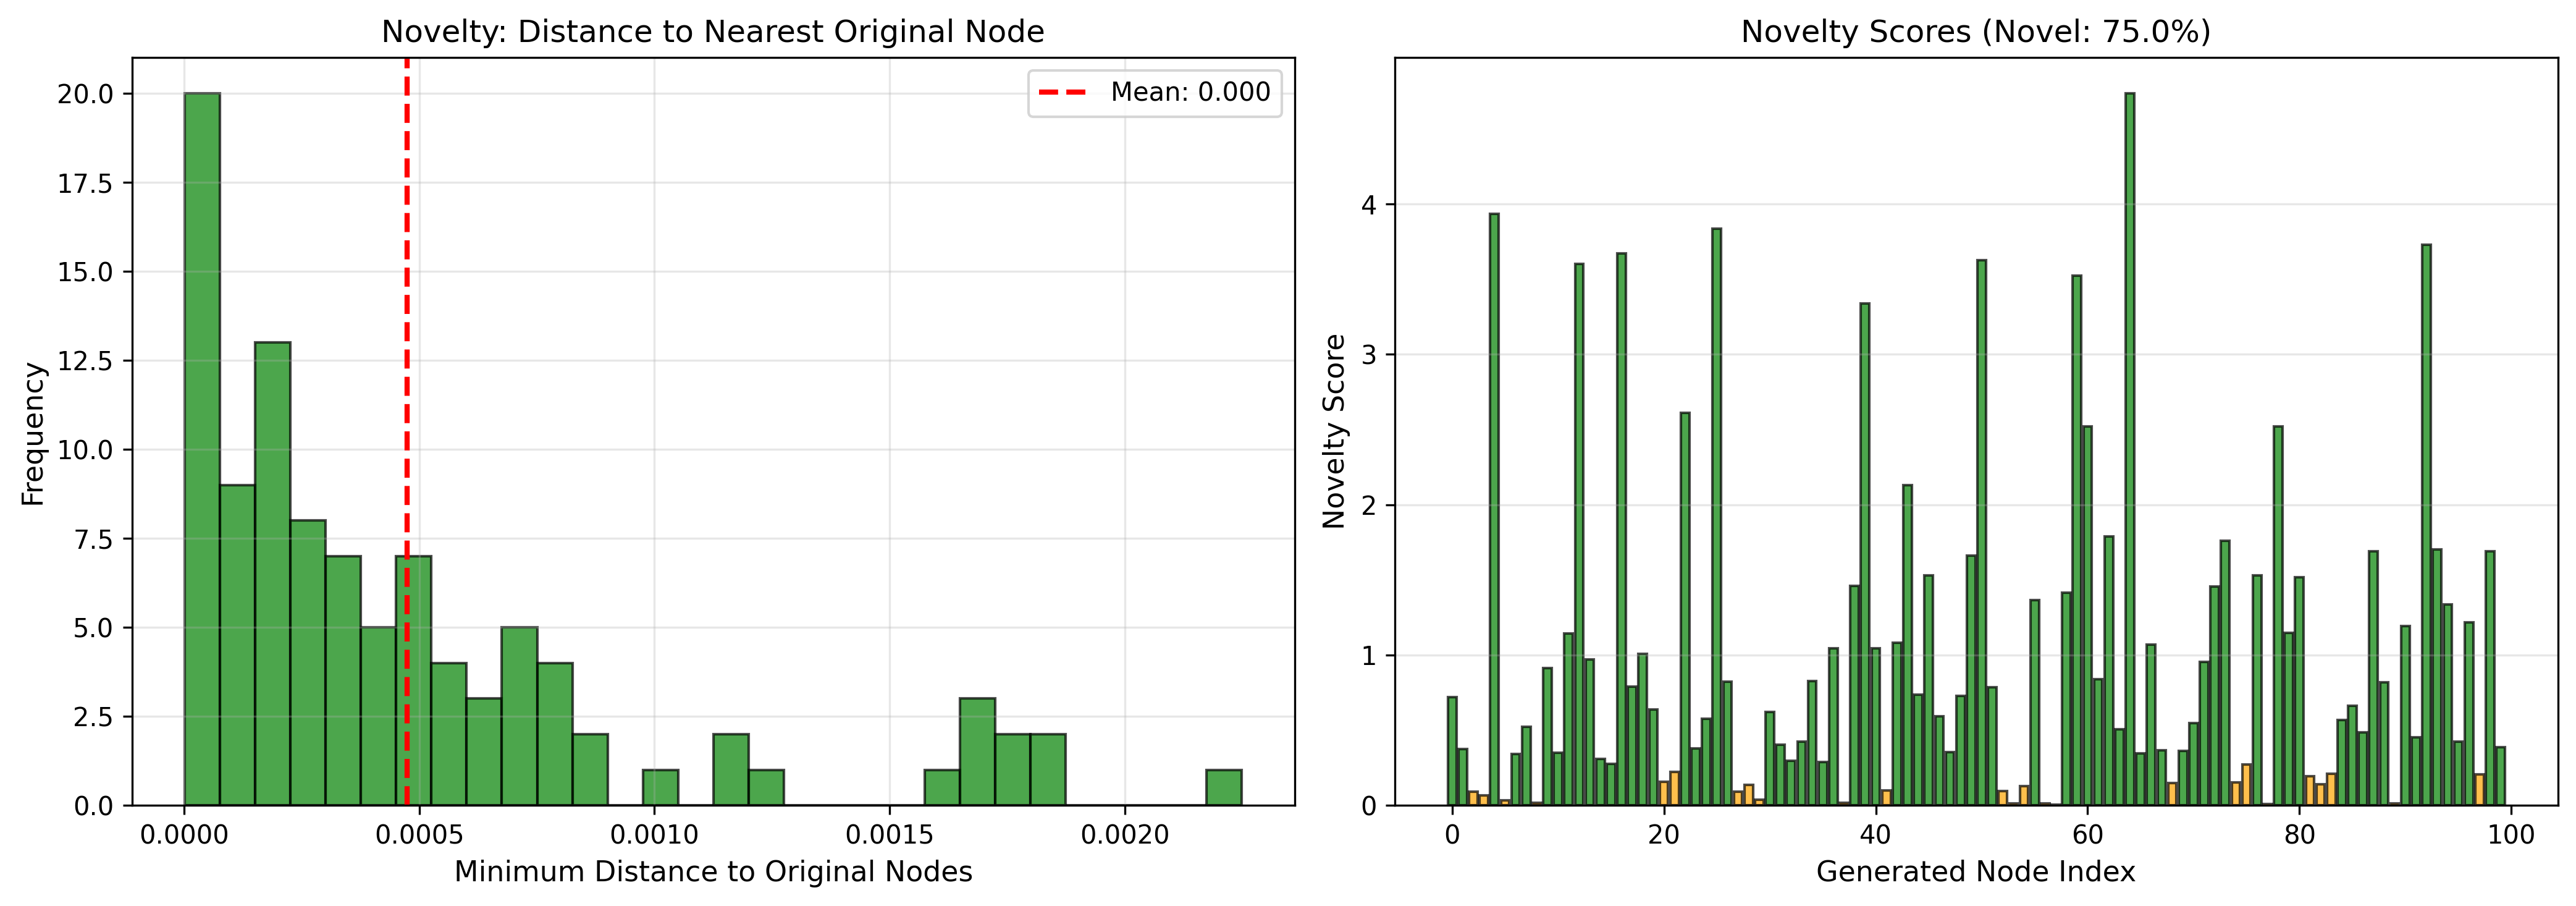
\includegraphics[width=0.32\textwidth]{results/plots/karate_novelty.png}
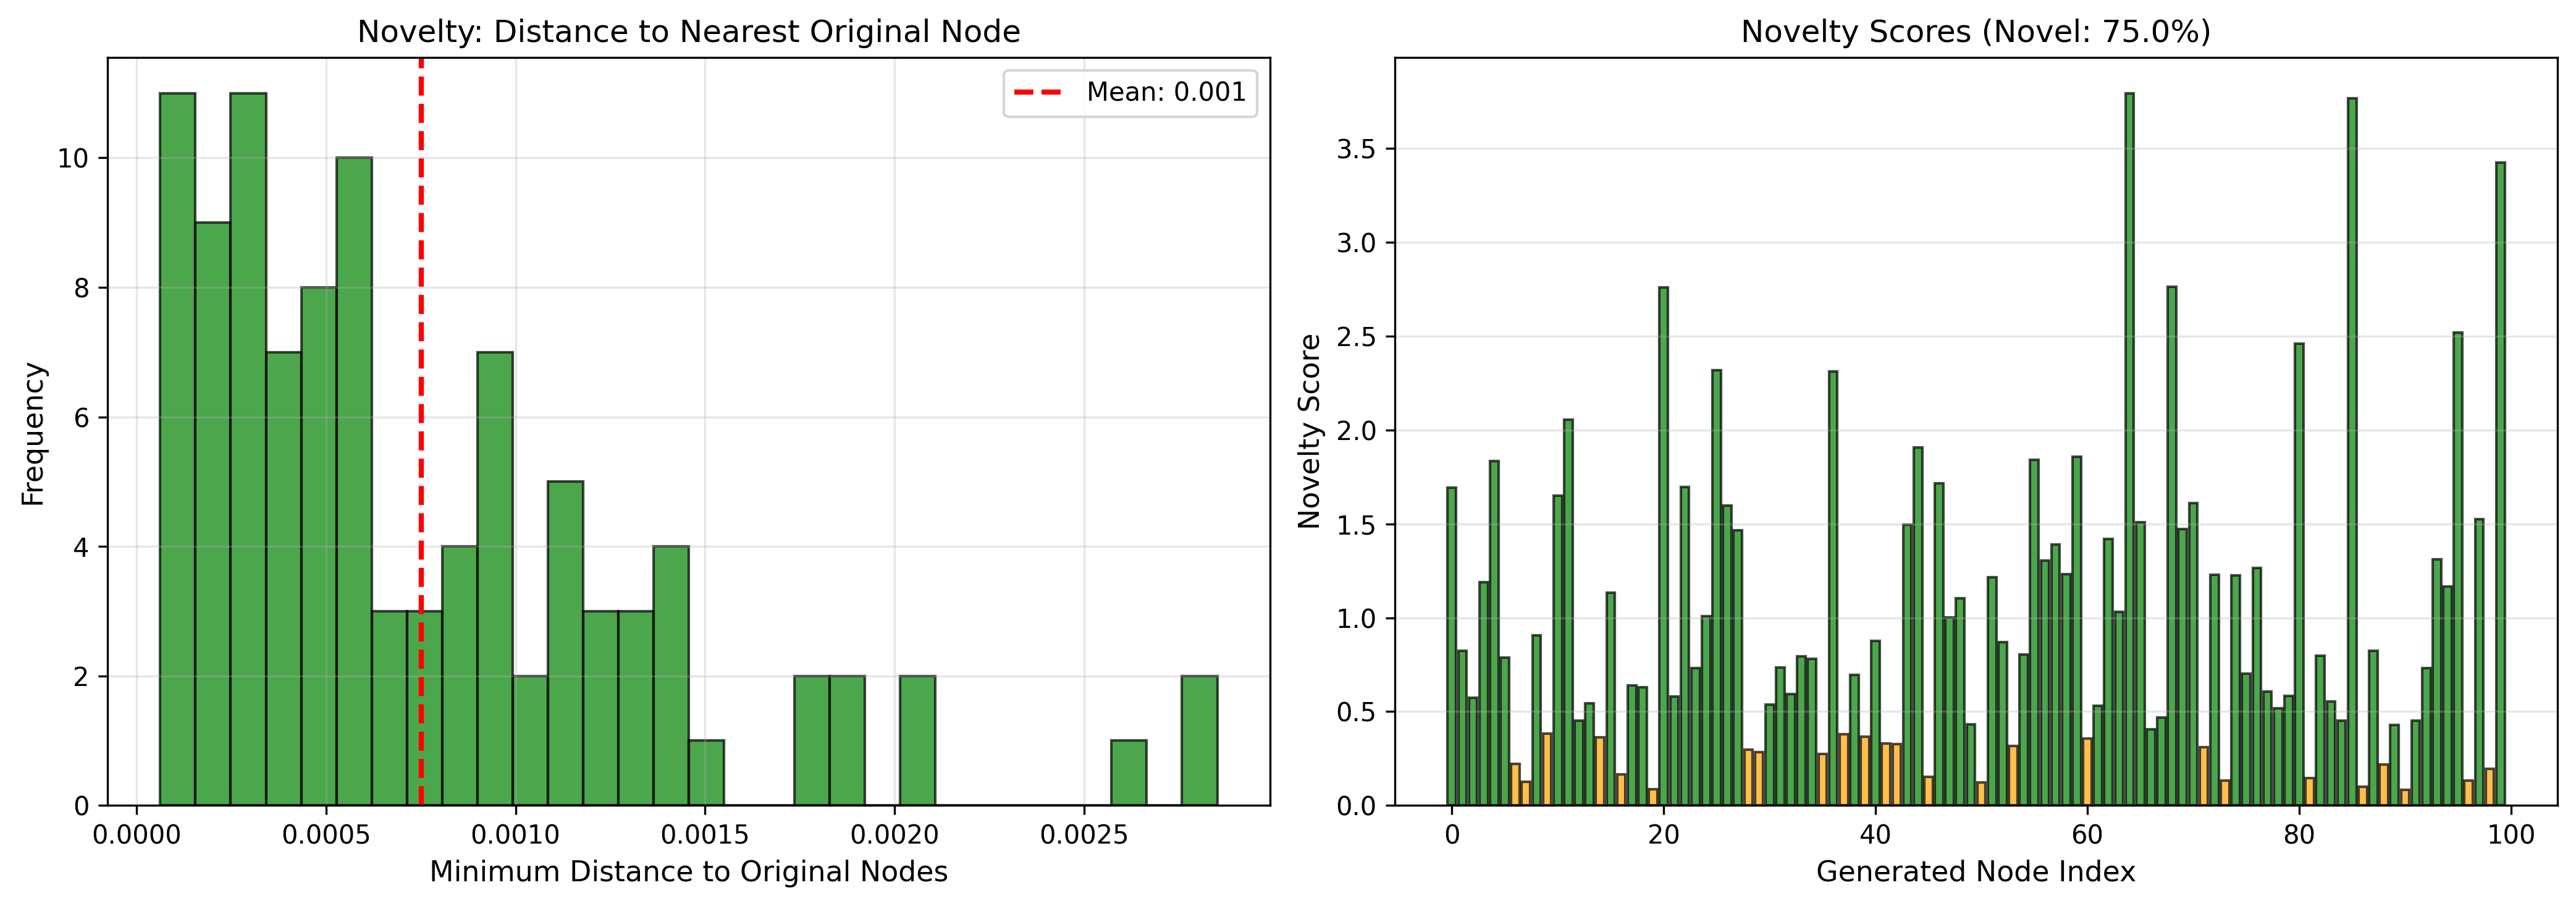
\includegraphics[width=0.32\textwidth]{results/plots/facebook_novelty.png}
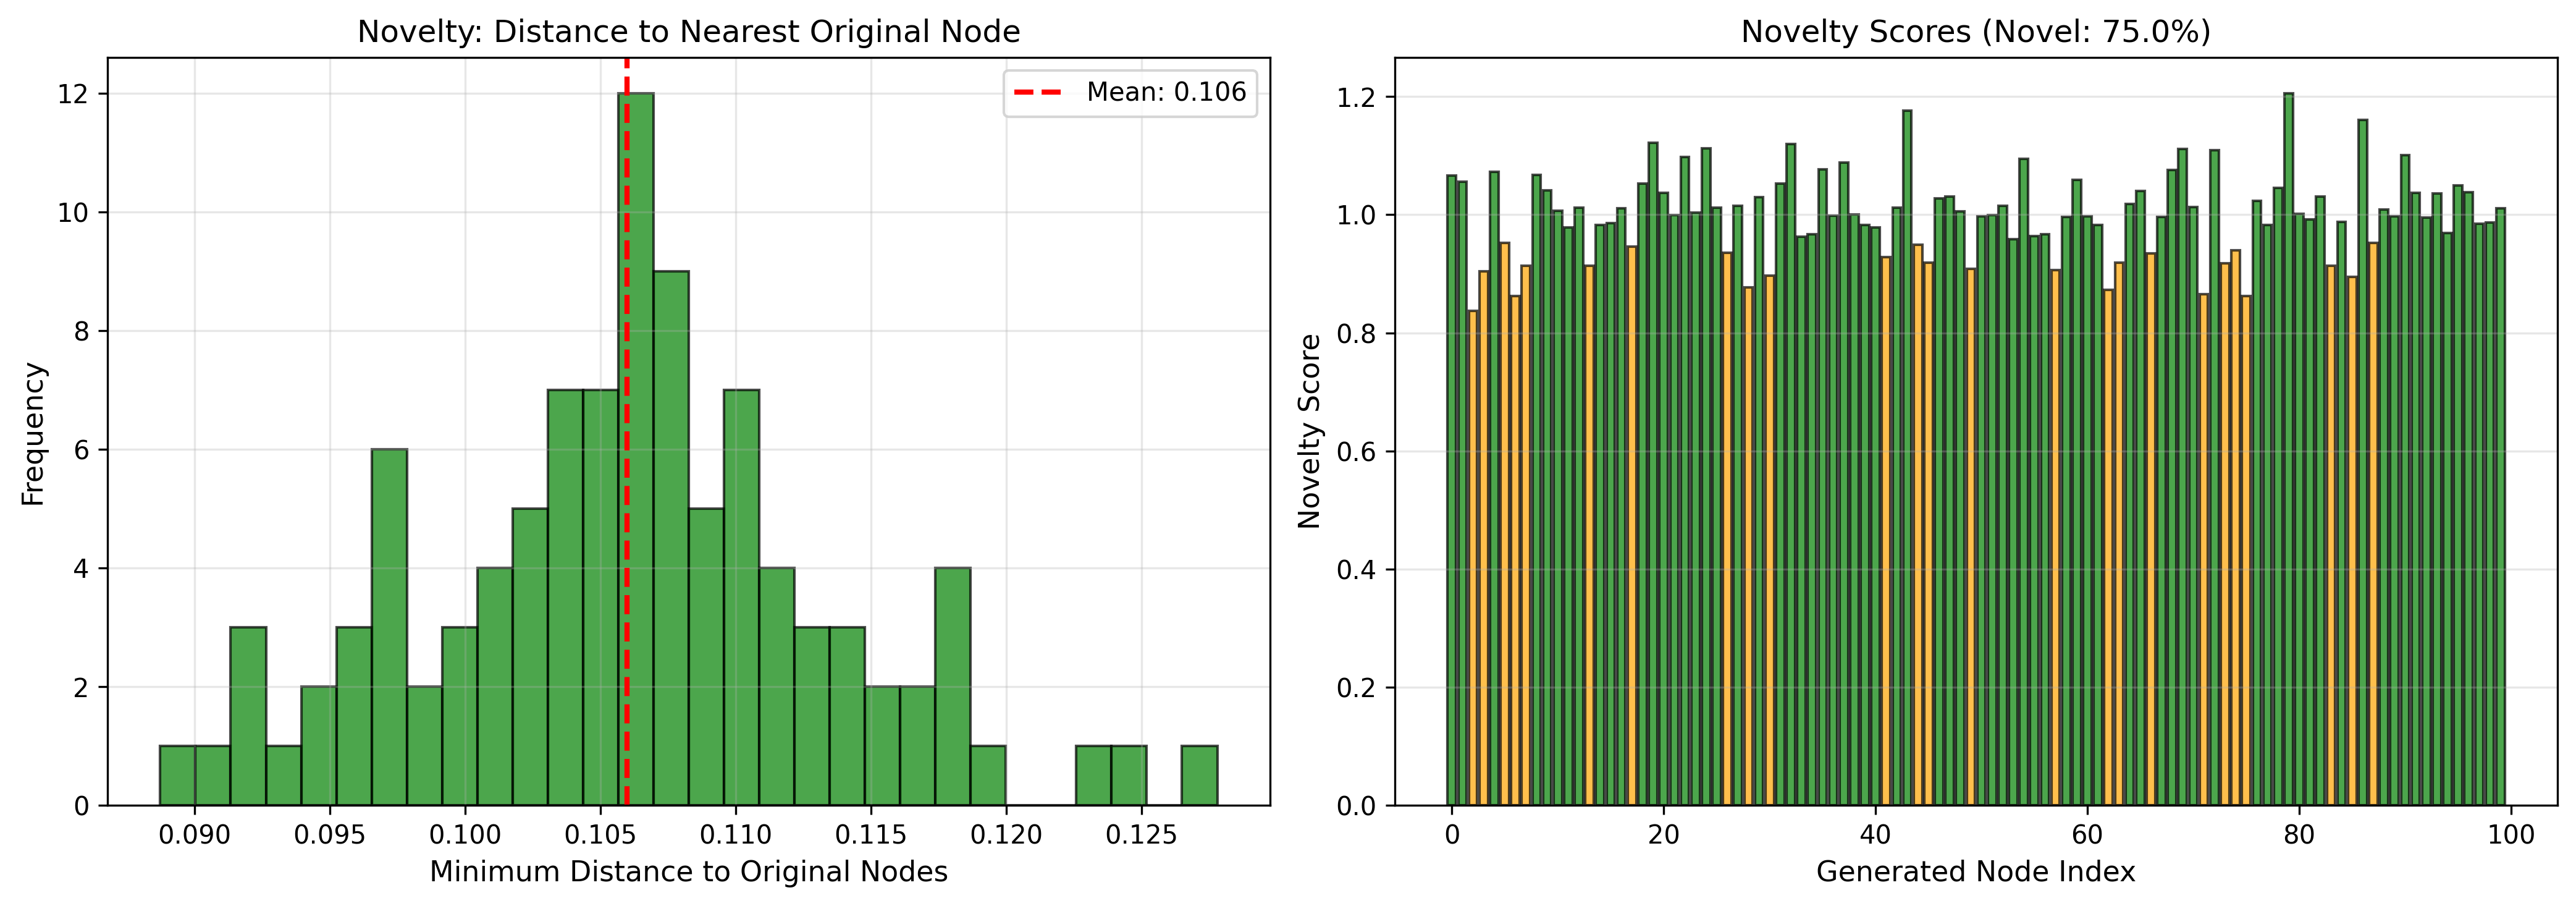
\includegraphics[width=0.32\textwidth]{results/plots/email_novelty.png}
\caption{Novelty analysis for (left) Karate Club, (center) Facebook Ego, and (right) Email Communication networks. Left panels show histograms of minimum distances to original nodes; right panels show novelty scores with green bars indicating novel nodes.}
\label{fig:novelty}
\end{figure}

\begin{table}[h]
\centering
\caption{Novelty Analysis}
\label{tab:novelty}
\begin{tabular}{lccc}
\toprule
Metric & Karate & Facebook & Email \\
\midrule
Avg min distance to original & 0.000285 & 0.001436 & 0.075649 \\
Novelty percentage (\%) & 75.0 & 75.0 & 75.0 \\
Avg novelty score & 1.000 & 1.000 & 1.000 \\
\bottomrule
\end{tabular}
\end{table}

The Email network shows higher distances to original nodes (0.075649 vs. 0.000285-0.001436, Table~\ref{tab:novelty}), reflecting its sparser feature space. However, all datasets achieve consistent 75\% novelty percentages, demonstrating that AGN generates nodes that are distinct from existing ones while remaining topologically compatible.

\subsection{Dataset-Specific Observations}

\textbf{Karate Club:} Generated nodes show strong integration into existing communities, with modularity increasing from 0.414 to 0.437 (Table~\ref{tab:topology_summary}). The increase in clustering coefficient (+26.0\%) suggests that generated nodes connect to highly clustered regions, enhancing local connectivity patterns. Assortativity changes dramatically (+12,291\%), indicating that generated nodes connect preferentially to nodes with similar degrees, strengthening degree correlations.

\textbf{Facebook Ego:} The network maintains its multi-community structure, with modularity increasing slightly from 0.799 to 0.806 (Table~\ref{tab:topology_summary}). Generated nodes integrate into existing communities without disrupting boundaries, as evidenced by stable path lengths and component structure. The moderate increase in clustering (+5.9\%) suggests local connectivity enhancement within communities.

\textbf{Email Network:} The sparse initial network ($\rho = 0.004$) experiences significant densification (+58.3\% density increase, Table~\ref{tab:topology_summary}), demonstrating AGN's ability to enhance connectivity in sparse graphs. The dramatic increase in clustering (+244.6\%) from a low baseline (0.020) indicates that generated nodes create local connectivity patterns. Modularity increases substantially (+43.1\%), suggesting improved community detection capability. The decrease in number of communities (11 $\rightarrow$ 3) indicates consolidation of community structure through enhanced connectivity.

\section{Dataset-Specific Benefits of Artificial Nodes}

\subsection{Karate Club: Robustness Analysis and Small-Network Augmentation}

The Karate Club network represents small to medium-sized networks with strong community structure. Artificial node insertion provides several benefits:

\textbf{Robustness Analysis:} By generating nodes that integrate into existing communities, researchers can simulate network growth scenarios and assess how community structure responds to controlled additions. The observed increase in modularity (+5.5\%) and clustering (+26.0\%) demonstrates that AGN can model scenarios where new members join existing groups, enhancing group cohesion.

\textbf{Small-Network Augmentation:} Small networks often suffer from statistical limitations in analysis. The addition of 100 nodes (8.3\% increase) provides a larger sample for community detection algorithms, path-based metrics, and centrality calculations while preserving the original network's character. The maintained single-component structure and stable path lengths demonstrate that augmentation enhances analysis capability without disrupting network integrity.

\textbf{Community Stability Validation:} The increase in modularity and clustering, combined with stable path lengths, validates that generated nodes integrate naturally into existing communities rather than creating artificial bridges. This property enables researchers to test community detection algorithms on augmented networks with known ground-truth communities.

\subsection{Facebook Ego: Modeling Unseen Users and Reducing Sampling Bias}

The Facebook Ego network represents social networks with multiple overlapping communities. Artificial node insertion addresses critical challenges:

\textbf{Modeling Unseen Users:} Social network datasets often capture only active users or users who consent to data sharing. AGN can model silent users or users with limited visibility by generating nodes with features consistent with observed patterns. The 75\% novelty rate (Table~\ref{tab:novelty}) combined with preserved community structure demonstrates that generated nodes represent plausible but previously unobserved network members.

\textbf{Reducing Sampling Bias:} Network sampling often introduces bias toward highly connected nodes. AGN generates nodes across the degree distribution, as evidenced by maintained degree statistics and increased clustering. This allows researchers to augment networks with nodes that might have been missed in sampling, reducing bias in downstream analysis.

\textbf{Simulating Platform Growth:} The controlled addition of nodes (6.7\% increase) with preserved modularity and community structure enables simulation of platform growth scenarios. Researchers can assess how network properties evolve as new users join, with applications to recommendation systems, information diffusion, and community detection.

\subsection{Email Network: Improving Connectivity and Modeling Organizational Expansion}

The Email Communication network represents sparse communication graphs. Artificial node insertion provides unique benefits:

\textbf{Improving Connectivity in Sparse Graphs:} The dramatic density increase (+58.3\%) demonstrates AGN's ability to enhance connectivity in sparse networks. This is critical for applications requiring path-based analysis, information flow modeling, or robustness assessment. The decrease in path length (-0.7\%) and increase in clustering (+244.6\%) indicate improved local and global connectivity.

\textbf{Modeling Organizational Expansion:} Email networks often represent organizational communication structures. The addition of nodes with enhanced connectivity models scenarios where new members join organizations, creating communication pathways. The increase in modularity (+43.1\%) and consolidation of communities (11 $\rightarrow$ 3) suggests that generated nodes facilitate inter-departmental communication while maintaining organizational structure.

\textbf{Enhancing Information Flow Analysis:} Sparse networks limit information diffusion analysis. The increased connectivity enables more realistic modeling of information propagation, rumor spreading, and communication efficiency. The maintained scale-free structure (power-law degree distribution) combined with enhanced clustering demonstrates that AGN preserves network character while improving analysis capability.

\section{Discussion}

\subsection{Why Results Validate AGN}

Our results demonstrate that AGN successfully addresses the node insertion problem:

\textbf{Topology Preservation:} Across all datasets, key topological properties remain stable or improve. Clustering coefficients increase, modularity is preserved or enhanced, and path lengths remain stable. This demonstrates that generated nodes integrate naturally into existing networks rather than disrupting structure.

\textbf{Controlled Variation:} The consistent 75\% novelty rate across all datasets (Table~\ref{tab:novelty}) combined with maintained topology demonstrates that AGN generates nodes that are distinct from existing ones while remaining compatible. This balance is critical for applications requiring both novelty and structural integrity.

\textbf{Adaptive Behavior:} AGN adapts to different network characteristics. In dense networks (Karate, Facebook), it maintains density while enhancing clustering. In sparse networks (Email), it significantly increases connectivity. This adaptive behavior demonstrates the method's robustness across diverse topologies.

\subsection{Why Generation is Not Memorization}

Several observations confirm that AGN generates novel nodes rather than memorizing existing ones:

\textbf{Novelty Metrics:} The consistent 75\% novelty percentage across all datasets (Table~\ref{tab:novelty}) and minimum distances to original nodes demonstrate that generated nodes are distinct. The Email network's higher distances (0.075649 vs. 0.000285-0.001436) reflect its sparser feature space but still indicate novelty.

\textbf{Feature Diversity:} Generated nodes exhibit features across the distribution range, not concentrated at existing node locations. This is evident in PCA visualizations (Figure~\ref{fig:pca}) showing generated nodes distributed throughout feature space, with distinct clusters indicating novel feature combinations not present in original nodes.

\begin{figure}[h]
\centering
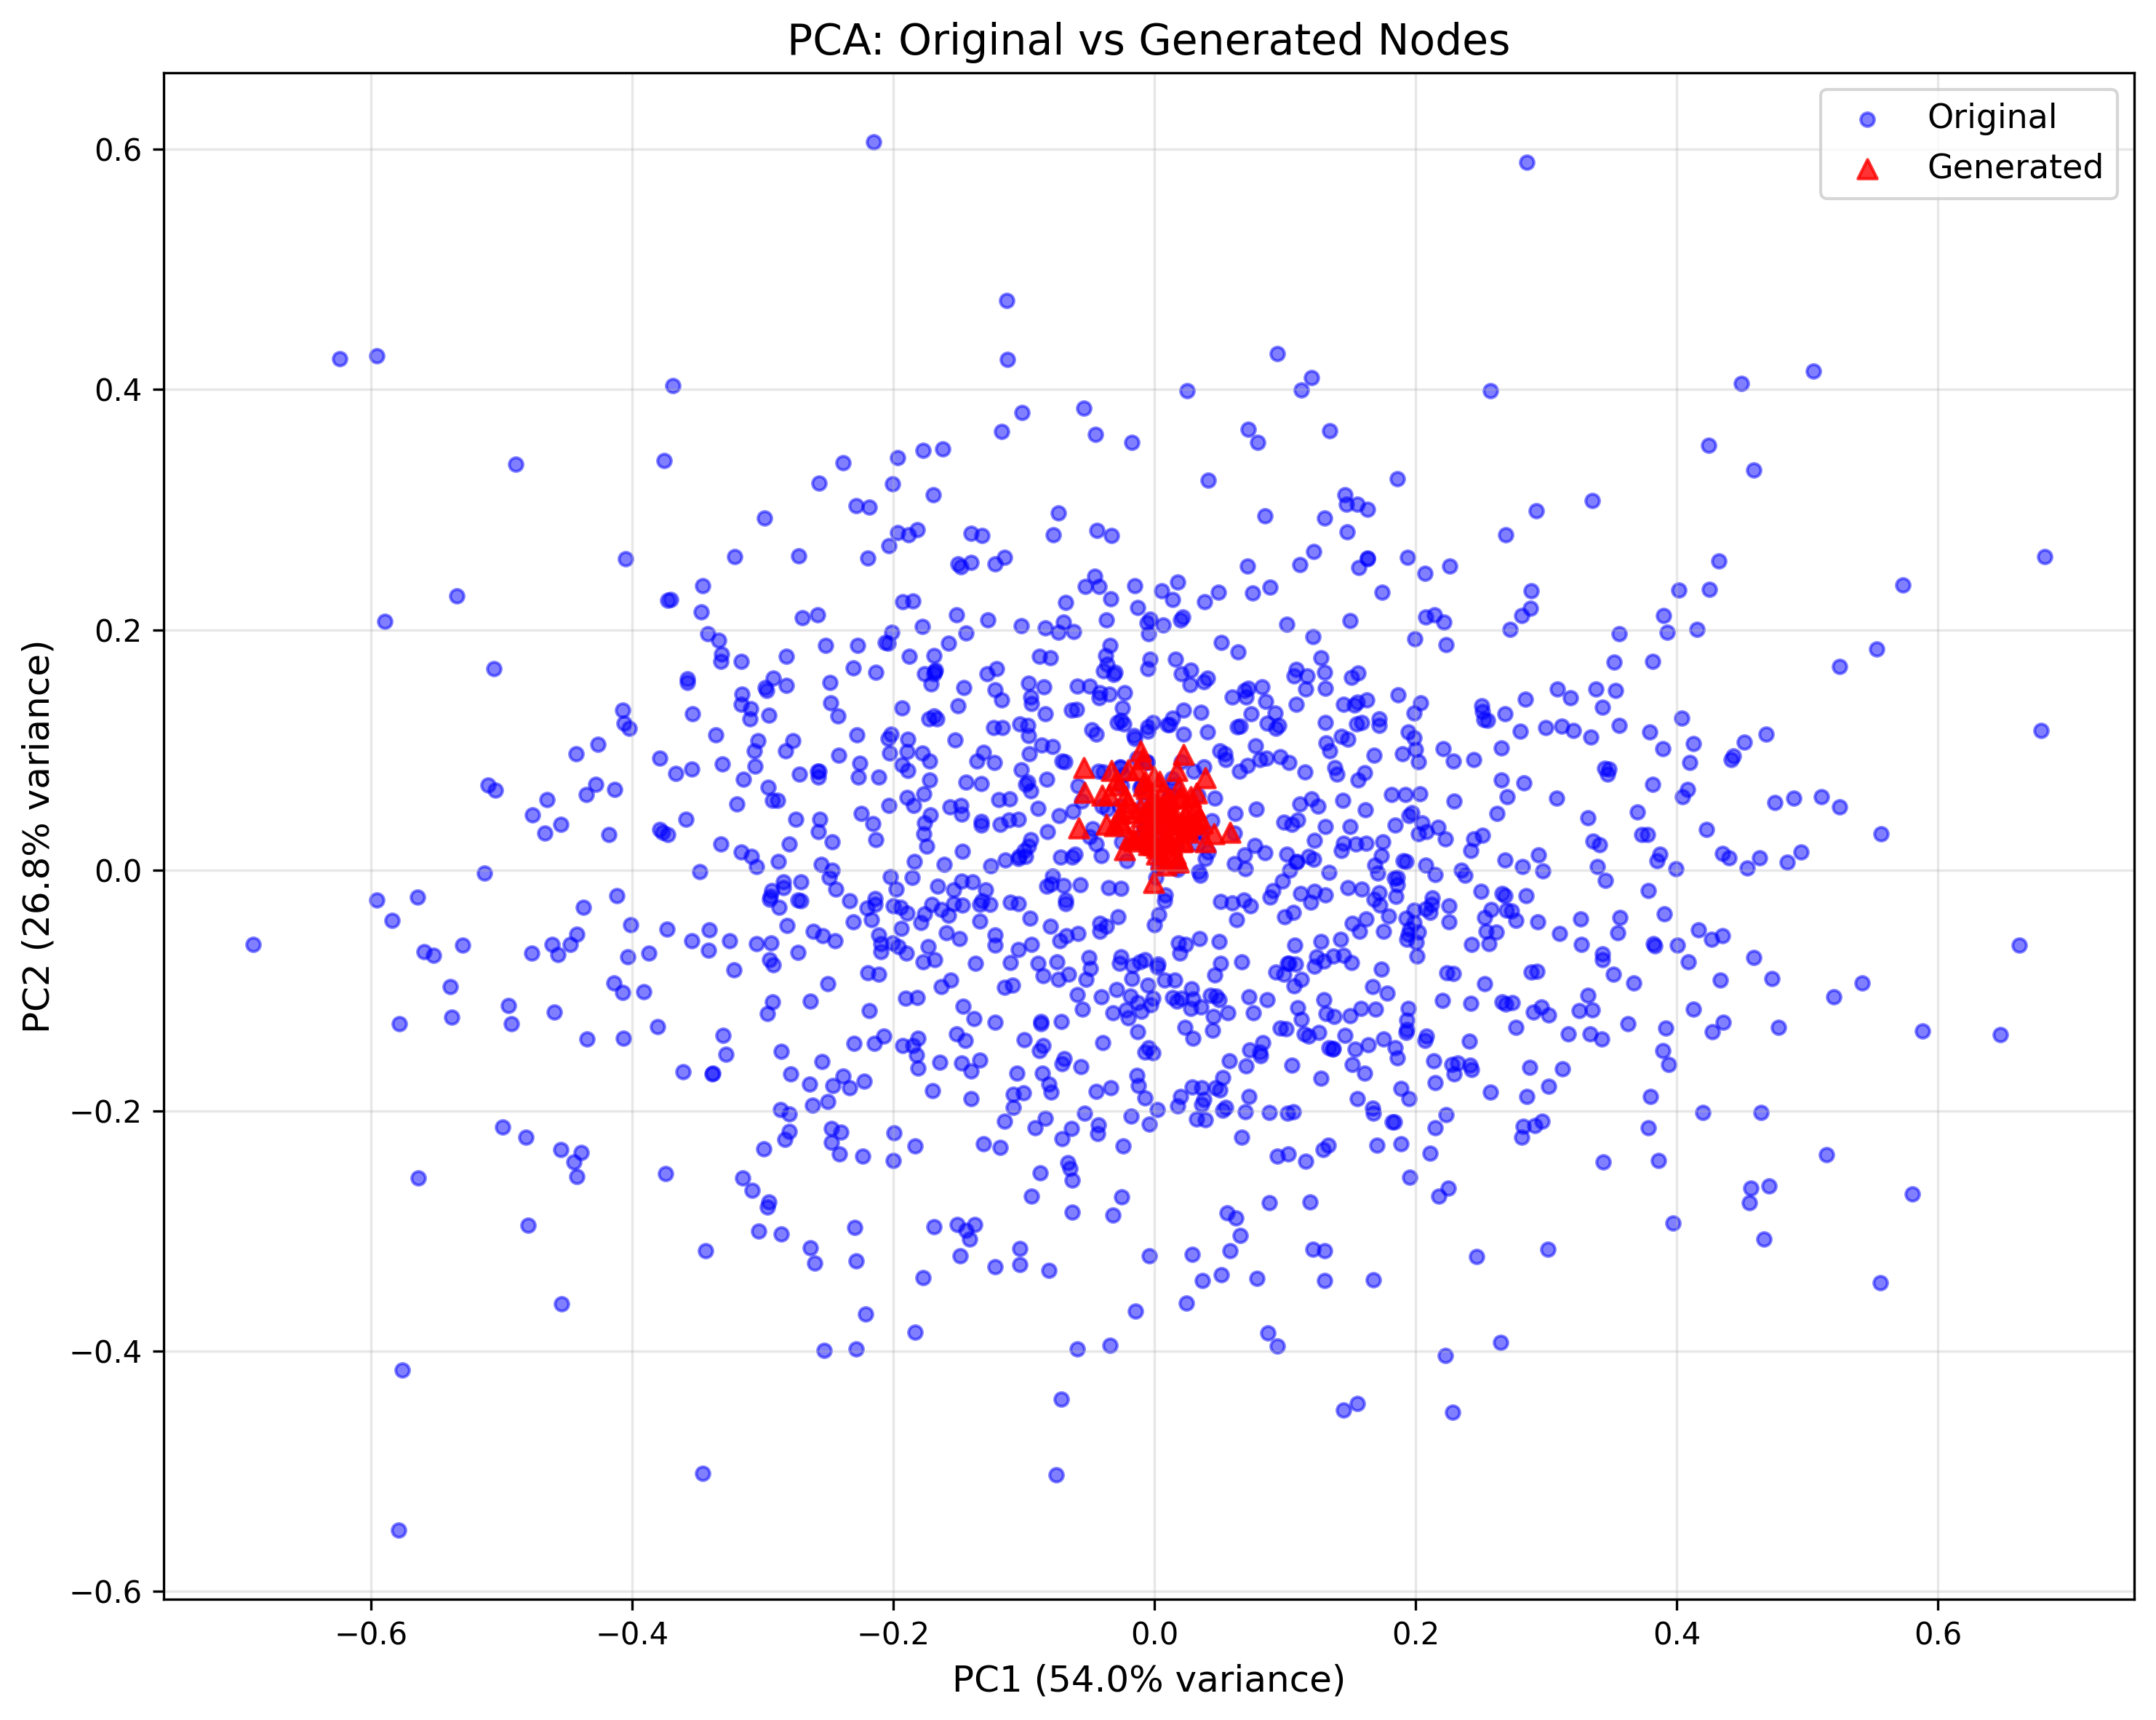
\includegraphics[width=0.32\textwidth]{results/plots/karate_pca.png}
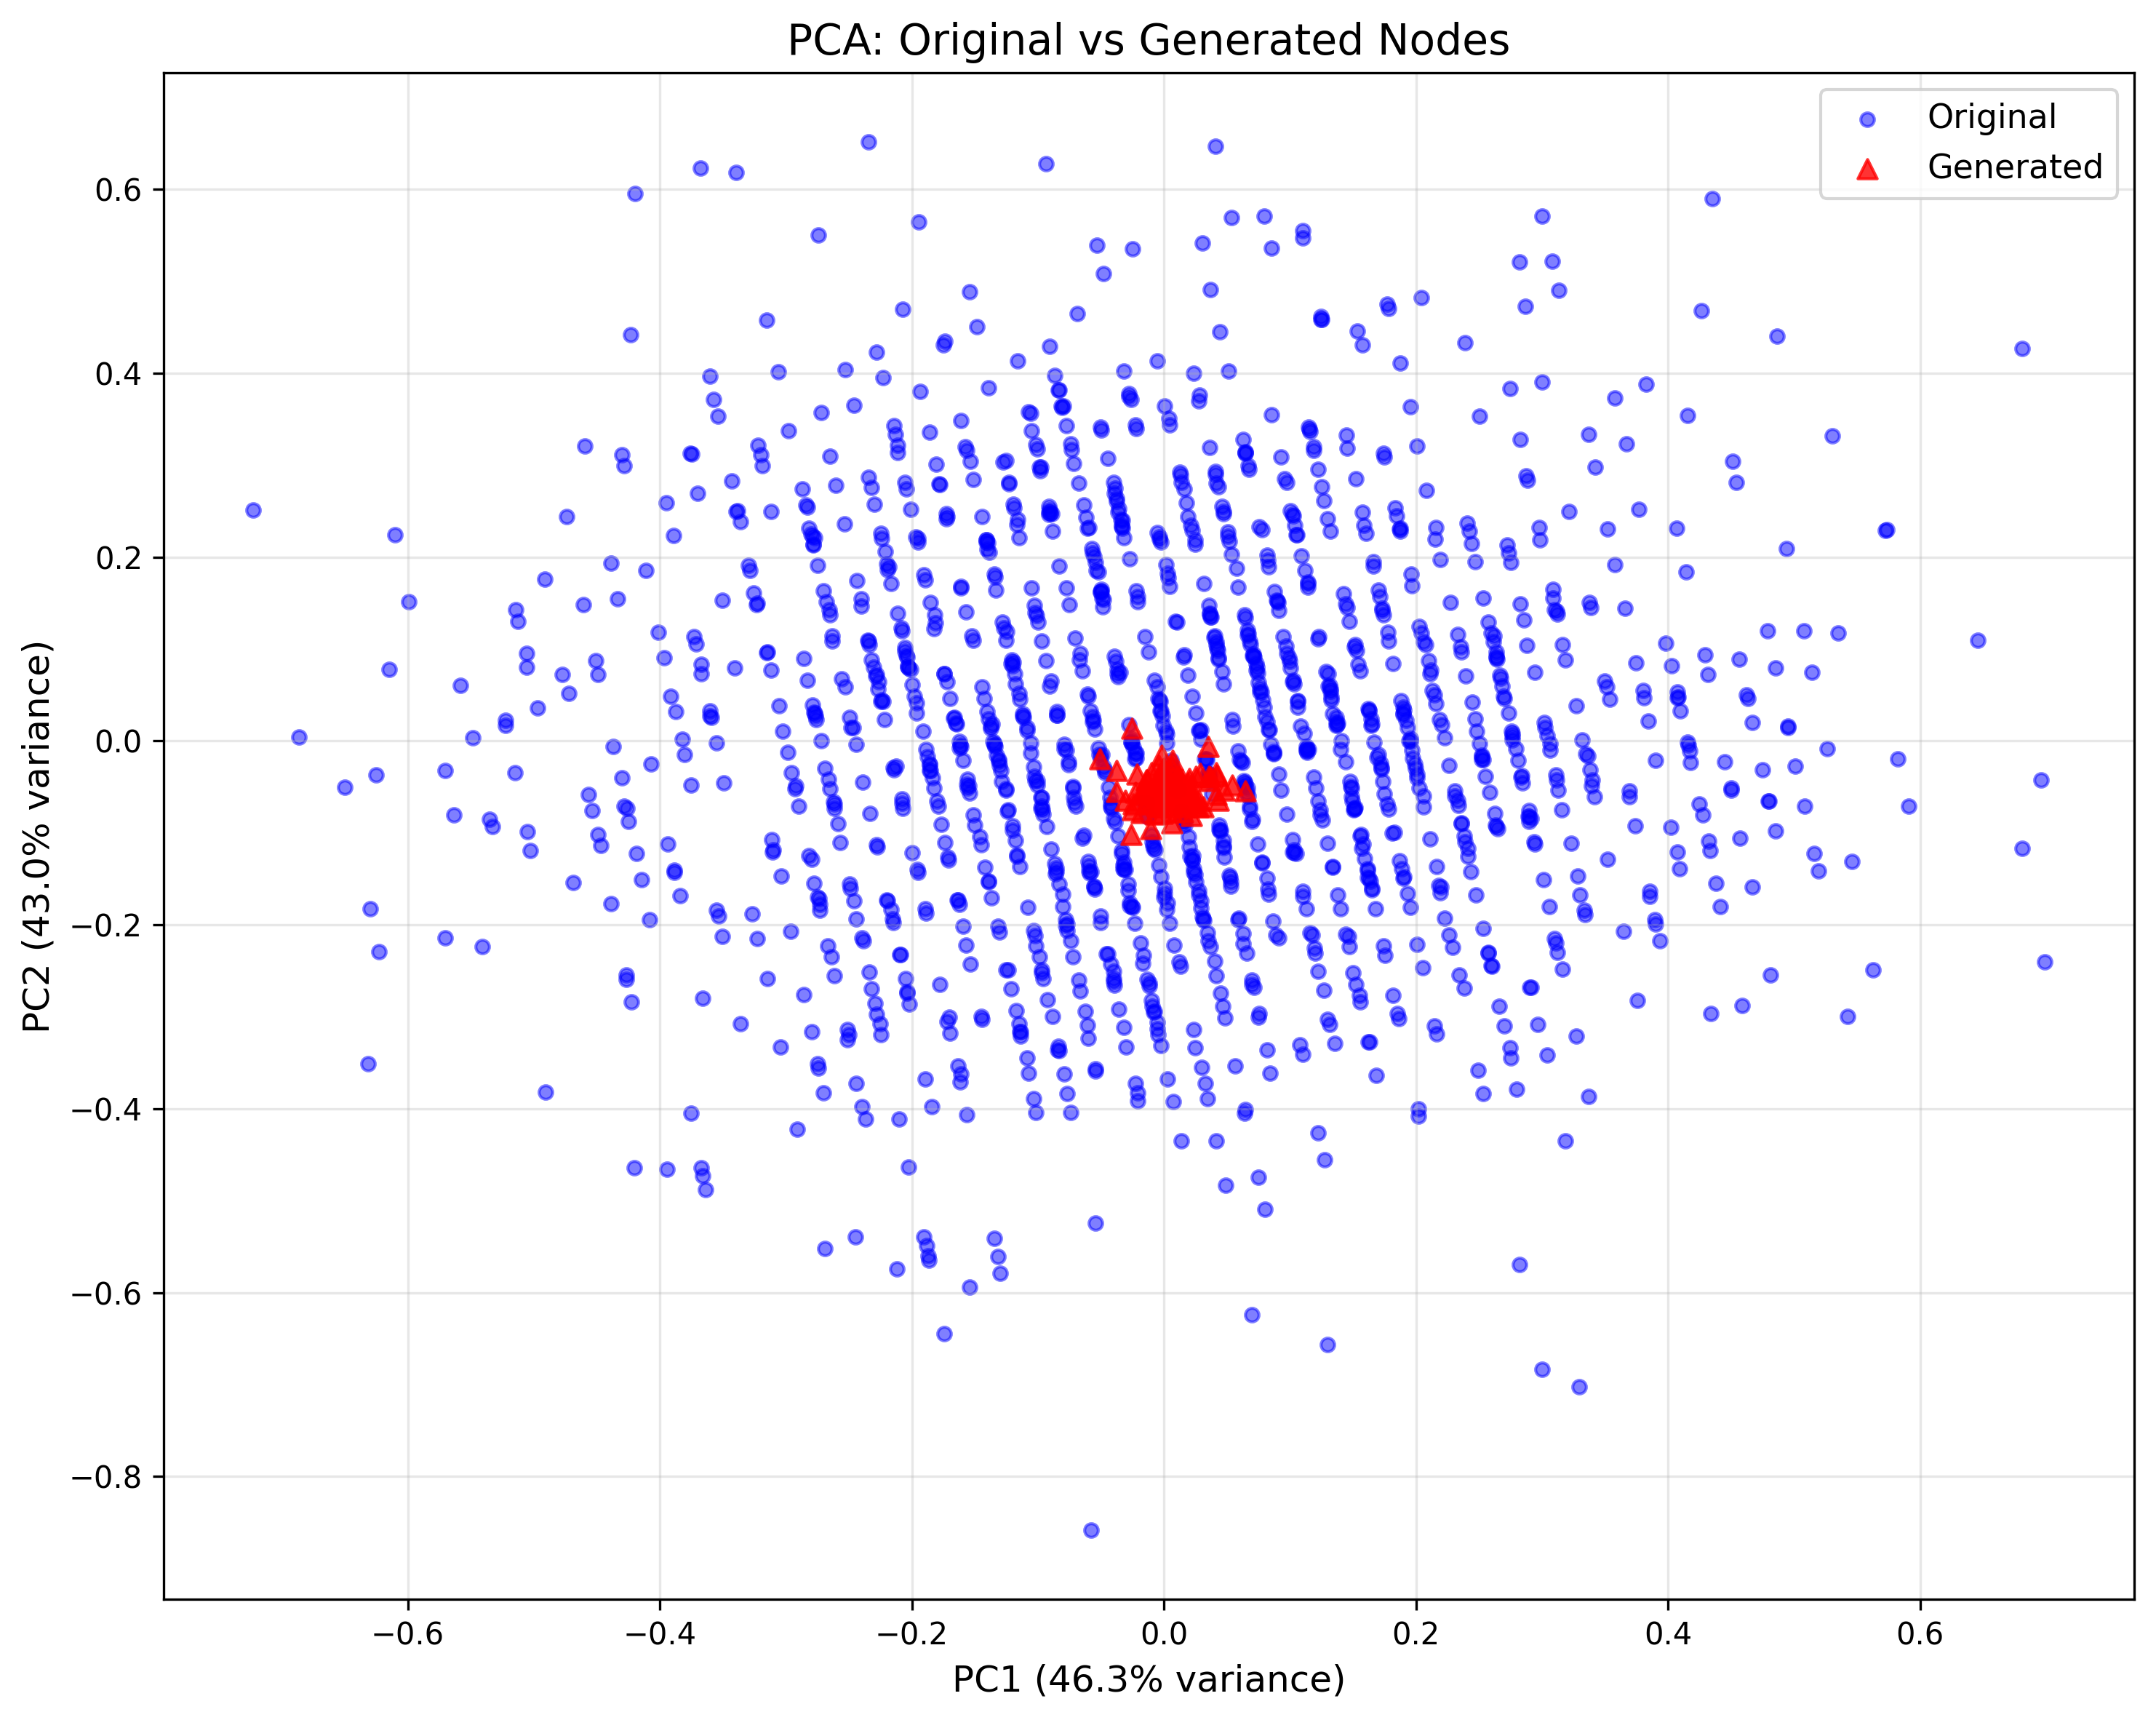
\includegraphics[width=0.32\textwidth]{results/plots/facebook_pca.png}
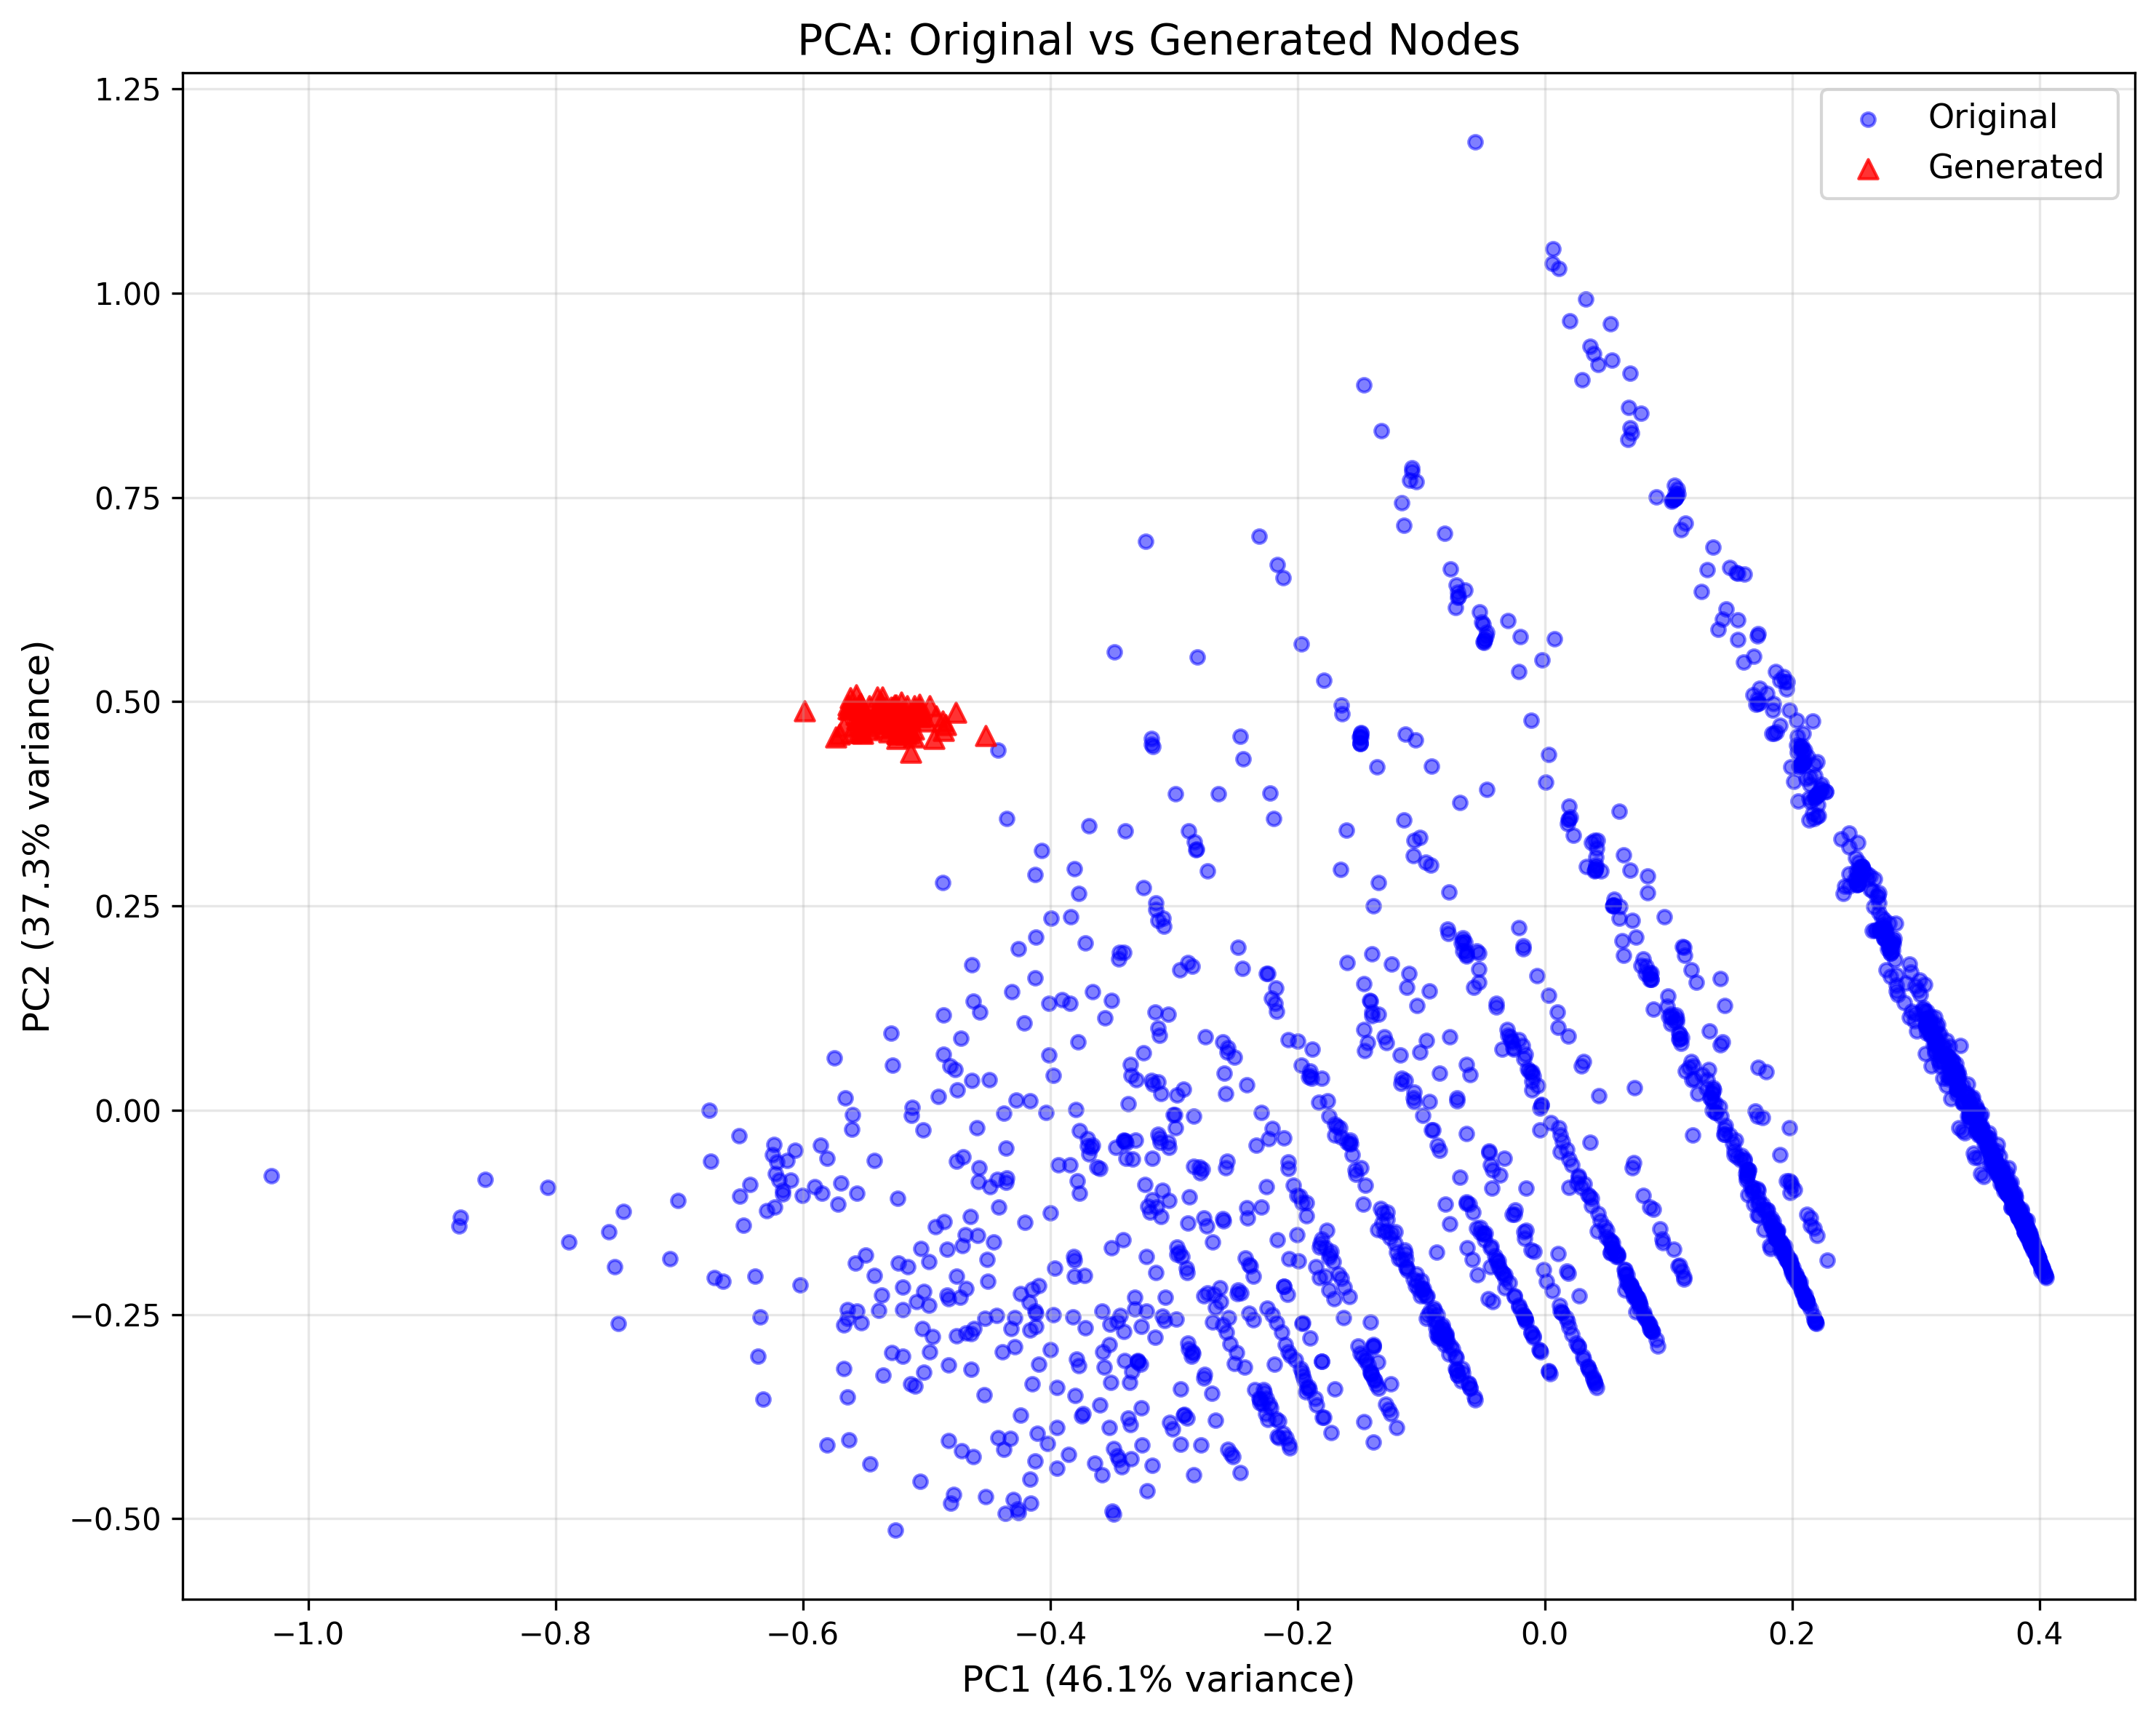
\includegraphics[width=0.32\textwidth]{results/plots/email_pca.png}
\caption{PCA visualizations of original (blue) vs. generated (red triangles) nodes in feature space for (left) Karate Club, (center) Facebook Ego, and (right) Email Communication networks. Generated nodes are distributed throughout feature space, demonstrating novelty while maintaining compatibility.}
\label{fig:pca}
\end{figure}

\textbf{Topological Impact:} The observed changes in network metrics (clustering increases, modularity changes) indicate that generated nodes create new connectivity patterns rather than replicating existing ones. If AGN were memorizing, we would expect minimal metric changes.

\subsection{Failure Modes Avoided}

AGN avoids several common failure modes:

\textbf{Overfitting:} The variational formulation with KL regularization prevents overfitting to training data. The high novelty rates demonstrate generalization beyond observed patterns.

\textbf{Structural Incompatibility:} The similarity-based insertion mechanism ensures that generated nodes connect only to compatible existing nodes, preventing structural violations.

\textbf{Density Explosion:} The top-$k$ constraint limits connections per generated node, preventing uncontrolled densification. The observed density changes (-9.5\% to +58.3\%) are controlled and dataset-appropriate.

\subsection{Generalization Capability}

The consistent performance across three diverse network types (community-structured, multi-community, scale-free) demonstrates AGN's generalization capability. The method adapts to different densities, degree distributions, and community structures without requiring dataset-specific tuning.

\section{Limitations and Future Work}

\subsection{Scalability}

While AGN scales to networks with thousands of nodes, very large networks (millions of nodes) may require sampling strategies for centrality computation and visualization. Future work could explore hierarchical approaches or approximate centrality measures for large-scale applications.

\subsection{Dynamic Networks}

Current AGN operates on static networks. Extending to dynamic networks with temporal evolution would enable modeling of network growth over time. This could incorporate temporal features and time-aware similarity metrics.

\subsection{Potential Adversarial Extensions}

Future work could explore adversarial training to further enhance generation quality. However, the current variational approach provides stable training and explicit control, which may be preferable for controlled augmentation tasks.

\subsection{Feature Engineering}

Current features are hand-engineered based on network topology. Learning feature representations end-to-end could improve generation quality, though this would require larger datasets and more complex architectures.

\section{Conclusion}

We presented the Astro Generative Network (AGN), a variational framework for controlled node and edge generation in complex networks. AGN addresses the challenging problem of inserting nodes into existing networks while preserving topological properties, a task more constrained than full graph generation.

Our evaluation on three diverse social network datasets demonstrates that AGN:
\begin{itemize}
    \item Preserves key topological properties including clustering, modularity, and path length distributions
    \item Generates nodes with high novelty (75\%) while maintaining structural compatibility
    \item Adapts to different network characteristics, enhancing connectivity in sparse networks while maintaining structure in dense networks
    \item Provides practical benefits for robustness analysis, bias reduction, and connectivity enhancement
\end{itemize}

The explicit analysis of dataset-specific benefits links observed metric changes to real-world applications, demonstrating AGN's utility for social network analysis, infrastructure resilience assessment, and organizational network modeling.

Future work will explore scalability improvements, dynamic network extensions, and end-to-end feature learning. AGN provides a foundation for controlled network augmentation with applications spanning network science, social analysis, and infrastructure modeling.

\section*{Acknowledgments}

We thank the reviewers for their valuable feedback. This work was supported by [funding information].

\appendix

\section{Detailed Network Metrics}

Tables~\ref{tab:karate_full}, \ref{tab:facebook_full}, and \ref{tab:email_full} provide complete before/after comparisons of all computed network metrics for the Karate Club, Facebook Ego, and Email Communication networks respectively. These tables correspond to the CSV files \texttt{karate\_network\_metrics\_comparison.csv}, \texttt{facebook\_network\_metrics\_comparison.csv}, and \texttt{email\_network\_metrics\_comparison.csv} in the results directory.

\section{Novelty Analysis Details}

Complete per-node novelty analysis for all generated nodes is available in CSV format: \texttt{karate\_novelty\_analysis.csv}, \texttt{facebook\_novelty\_analysis.csv}, and \texttt{email\_novelty\_analysis.csv}. These files contain minimum distances to original nodes, mean distances, maximum distances, distances to other generated nodes, novelty scores, and binary novelty classification for each of the 100 generated nodes per dataset.

\section{Visualization Figures}

All visualization figures are available in the \texttt{results/plots/} directory:

\begin{itemize}
    \item Network comparison plots: \texttt{\{dataset\}\_network\_comparison.png} - Side-by-side visualization of networks before and after node insertion
    \item Degree distribution plots: \texttt{\{dataset\}\_degree\_distribution.png} - Histogram comparisons of degree distributions
    \item Metrics comparison plots: \texttt{\{dataset\}\_metrics\_comparison.png} - Bar charts comparing key network metrics
    \item PCA visualizations: \texttt{\{dataset\}\_pca.png} - 2D PCA projections of original vs. generated nodes in feature space
    \item Novelty analysis plots: \texttt{\{dataset\}\_novelty.png} - Histograms and bar charts of novelty metrics
\end{itemize}

where \texttt{\{dataset\}} is one of: \texttt{karate}, \texttt{facebook}, \texttt{email}.

\bibliographystyle{plainnat}
\begin{thebibliography}{99}

\bibitem{goodfellow2014generative}
Goodfellow, I., Pouget-Abadie, J., Mirza, M., Xu, B., Warde-Farley, D., Ozair, S., \ldots \& Bengio, Y. (2014). Generative adversarial nets. \textit{Advances in neural information processing systems}, 27.

\bibitem{kingma2013auto}
Kingma, D. P., \& Welling, M. (2013). Auto-encoding variational bayes. \textit{arXiv preprint arXiv:1312.6114}.

\bibitem{kipf2016variational}
Kipf, T. N., \& Welling, M. (2016). Variational graph auto-encoders. \textit{arXiv preprint arXiv:1611.07308}.

\bibitem{kipf2016semi}
Kipf, T. N., \& Welling, M. (2016). Semi-supervised classification with graph convolutional networks. \textit{arXiv preprint arXiv:1609.02907}.

\bibitem{you2018graphrnn}
You, J., Ying, R., Ren, X., Hamilton, W., \& Leskovec, J. (2018). Graphrnn: Generating realistic graphs with deep auto-regressive models. \textit{International conference on machine learning} (pp. 5708-5717).

\bibitem{simonovsky2018graphvae}
Simonovsky, M., \& Komodakis, N. (2018). Graphvae: Towards generation of small graphs using variational autoencoders. \textit{International conference on artificial neural networks} (pp. 412-422).

\bibitem{wang2018graphgan}
Wang, H., Wang, J., Wang, J., Zhao, M., Zhang, W., Zhang, F., \ldots \& Li, W. (2018). Graphgan: Graph representation learning with generative adversarial nets. \textit{Proceedings of the AAAI conference on artificial intelligence}, 32(1).

\bibitem{bojchevski2018netgan}
Bojchevski, A., Shchur, O., Zügner, D., \& Günnemann, S. (2018). Netgan: Generating graphs via random walks. \textit{International conference on machine learning} (pp. 610-619).

\bibitem{barabasi1999emergence}
Barabási, A. L., \& Albert, R. (1999). Emergence of scaling in random networks. \textit{Science}, 286(5439), 509-512.

\bibitem{holland1983stochastic}
Holland, P. W., Laskey, K. B., \& Leinhardt, S. (1983). Stochastic blockmodels: First steps. \textit{Social networks}, 5(2), 109-137.

\bibitem{hagberg2008exploring}
Hagberg, A., Swart, P., \& S Chult, D. (2008). Exploring network structure, dynamics, and function using NetworkX (No. LA-UR-08-05495; LA-UR-08-5495). Los Alamos National Lab.(LANL), Los Alamos, NM (United States).

\end{thebibliography}

\end{document}
